% Layout adapted from template/bmo_original_main.tex; the original is preserved.
\documentclass[12pt,a4paper,oneside]{report}
\title{\textbf{OLS Regression Lecture Notes}\\[0.5em]\large Interpretation, Goodness of Fit, and Unbiasedness}
\author{\textit{Jintian}-JTST}
\date{Weeks 2--4\\20 October 2026}
\usepackage{geometry}
\geometry{a4paper,left=2cm,right=2cm,top=2cm,bottom=2cm}
\usepackage{amsmath,amssymb,amsthm}
\usepackage[english]{babel}
\usepackage[UTF8,scheme=plain,fontset=windows]{ctex}
\usepackage{indentfirst,graphicx,float}
\usepackage[table]{xcolor}
\usepackage{booktabs,longtable,array}
\usepackage{enumitem}
\usepackage{hyperref}
\usepackage{bookmark}
\hypersetup{unicode=true,colorlinks=true,linkcolor=black,urlcolor=blue!55!black,citecolor=blue!55!black,pdftitle={OLS Regression Notes - Weeks 2-4},pdfauthor={Jintian-JTST},bookmarksnumbered=true}
\graphicspath{{figures/}{qa/source-crops/}}
\theoremstyle{definition}
\newtheorem{definition}{Definition}[section]
\newtheorem{theorem}{Theorem}[section]
\newtheorem{lemma}[theorem]{Lemma}
\newtheorem{example}{Example}[section]
\newtheorem{exercise}{Exercise}[section]
\definecolor{noteYellow}{RGB}{244,245,128}
\definecolor{notePink}{RGB}{249,220,237}
\definecolor{noteBlue}{RGB}{33,54,118}
\definecolor{noteRed}{RGB}{153,39,43}
\newcommand{\hy}[1]{\begingroup\setlength{\fboxsep}{1.4pt}\colorbox{noteYellow}{\strut #1}\endgroup}
\newcommand{\hp}[1]{\begingroup\setlength{\fboxsep}{1.4pt}\colorbox{notePink}{\strut #1}\endgroup}
\newcommand{\hm}[1]{\begingroup\setlength{\fboxsep}{3pt}\colorbox{noteYellow}{$\displaystyle #1$}\endgroup}
\newcommand{\blue}[1]{{\color{noteBlue}#1}}
\newcommand{\red}[1]{{\color{noteRed}#1}}
\newcommand{\added}[1]{\par\smallskip\noindent{\small\color{noteBlue}\textbf{补充：}#1}}
\newcommand{\sourcepage}[3]{\par\phantomsection\label{src:w#1p#2}% PDF #2, handwritten #3
}
\newcommand{\corr}[1]{\unskip\nobreak\hspace{.08em}\hyperref[err:#1]{\textsuperscript{\color{noteRed}\scriptsize 勘误}}}
\newcommand{\E}{\operatorname{E}}
\newcommand{\Var}{\operatorname{Var}}
\newcommand{\Cov}{\operatorname{Cov}}
\newcommand{\Corr}{\operatorname{Corr}}
\newcommand{\RSS}{\operatorname{RSS}}
\newcommand{\ESS}{\operatorname{ESS}}
\newcommand{\TSS}{\operatorname{TSS}}
\newcommand{\educ}{\mathrm{educ}}
\newcommand{\wage}{\mathrm{wage}}
\newcommand{\hsGPA}{\mathrm{hsGPA}}
\newcommand{\colGPA}{\mathrm{colGPA}}
\newcommand{\ACT}{\mathrm{ACT}}
\newcolumntype{P}[1]{>{\raggedright\arraybackslash}p{#1}}
\setlist{itemsep=3pt,topsep=5pt}
\setlength{\emergencystretch}{2em}
\setlength{\parskip}{0.25em}
\setcounter{tocdepth}{2}
\setcounter{secnumdepth}{3}
\begin{document}
\maketitle
\pagenumbering{roman}
\tableofcontents
\clearpage
\chapter*{整理说明}
\addcontentsline{toc}{chapter}{整理说明}
本笔记依据 Week 2--4 的三份手写扫描稿整理，共 23 页。保留英文正文、中文批注、原有例题与证明的顺序；黄色和粉色重点、红蓝说明按原稿用途保留。版式直接沿用既有 BMO CAMP 笔记的 \texttt{report} 模板。

正文采用核对后的写法；实质修正旁的\corr{notation}链接可跳转至\hyperref[app:errata]{勘误与补充说明}。新增的必要解释标为“补充”。\hyperref[app:sources]{原稿对应表}可按原稿页码定位正文。原始扫描文件原样保存在项目的 \texttt{sources} 目录中。

图形均以 Python/Matplotlib 重画。无原始观测数据的图为\textbf{教学示意图}，不代表真实样本；带数值的拟合优度图由示意数据实际计算所得。纸张商标、扫描水印和印刷联系信息留在原稿副本，不作为课程内容重新排版。

\paragraph{Notation.} $\beta_j$ denotes a fixed population parameter; $\hat\beta_j$ is an OLS estimator (or its realised value when the sample is fixed). $u_i$ is the population error and $\hat u_i=y_i-\hat y_i$ is the fitted residual. Sample covariance, variance and correlation carry an explicit subscript $n$ when a distinction matters. $k$ counts regressors \emph{excluding} the intercept; $n$ is the sample size.

\clearpage
\pagenumbering{arabic}
\setcounter{chapter}{1}
\chapter{Interpretation of OLS Regression}
\label{ch:week2}
\section{Simple Ordinary Least Squares}
\sourcepage{2}{1}{2/1}
\label{sec:simple-interpretation}
\subsection{Model and the ceteris paribus interpretation}
The simple regression model is
\begin{equation}\label{eq:simple-model}
 y_i=\beta_0+\beta_1x_i+u_i.
\end{equation}
For another observation, $y_{i'}=\beta_0+\beta_1x_{i'}+u_{i'}$. 不同 observation 对应不同的 $u$；因此不能只因 $x$ 不同就把 $y$ 的全部变化归于 $x$。
Subtracting the two equations gives
\[\hm{\Delta y=\beta_1\Delta x+\Delta u}.\]
If $u$ does not change, $y$ changes by $\beta_1$ times the change in $x$:
\[\Delta u=0\quad\Longrightarrow\quad
\hy{$\Delta y=\beta_1\Delta x$},\qquad
\beta_1=\frac{\Delta y}{\Delta x}\quad(\Delta x\ne0).\]
\textbf{Interpretation.} \hy{Other factors being equal}, one unit increase in $x$ is associated with a $\beta_1$ unit increase in $y$. $\beta_1$ is the \hy{marginal effect of $x$ on $y$} in this linear model when $u$ is held fixed. 如果系数为负，应将“increase”读作相应的减少。

\subsection{Assumptions about the error}
\begin{enumerate}
\item \hy{$\E[u]=0$}: 均值为零。With an unrestricted intercept this can be achieved by normalisation. If $\E[u]=\alpha$, let $\varepsilon=u-\alpha$; then $\E[\varepsilon]=0$ and
\[y=\beta_0+\beta_1x+u=(\beta_0+\alpha)+\beta_1x+\varepsilon.\]
The intercept absorbs the nonzero mean; this does not by itself establish exogeneity.\corr{mean-normalisation}
\item \hy{Zero Conditional Mean (ZCM)}，零条件均值假设：
\begin{equation}\label{eq:zcm-simple}
\hm{\E[u\mid x]=0}.
\end{equation}
The expected value of $u$ does not depend on the value of $x$. With the first normalisation, $\E[u\mid x]=\E[u]=0$. 原稿亦称其为 \hy{exogeneity assumption}（外生性假设）。
\end{enumerate}
\begin{example}[Education and wages]
\[\wage=\beta_0+\beta_1\educ+u.\]
Unobserved factors include intelligence, family background, experience, training, etc. 在 ZCM 下，教育是 12 年还是 16 年，未观测因素 $u$ 的\emph{条件平均值}都相同；不是说每个人的能力和背景完全相同。
\blue{现实中很难控制所有未观测因素。}能力、背景可能与教育相关，因此这个假设并非天然合理。\red{Random assignment 可以帮助建立外生性}，但仍须结合实际研究设计核查。
\end{example}
% The rest of this chapter is appended after the GPA example below.

\subsection{Population regression function and fitted regression line}
\sourcepage{2}{2}{2/2}
Under \eqref{eq:zcm-simple}, the \hy{population regression function (PRF)}（总体回归函数）is
\begin{align}
\E[y\mid x]
&=\E[\beta_0+\beta_1x+u\mid x] \notag\\
&=\E[\beta_0+\beta_1x\mid x]+\E[u\mid x] \notag\\
&=\hm{\beta_0+\beta_1x}.\label{eq:prf}
\end{align}
给定 $x$ 后，$\beta_0+\beta_1x$ 为常数。$\beta_0$ is the intercept and $\beta_1$ is the slope of the PRF. The PRF is linear in $x$ in this simple level--level specification.
\begin{figure}[htbp]
\centering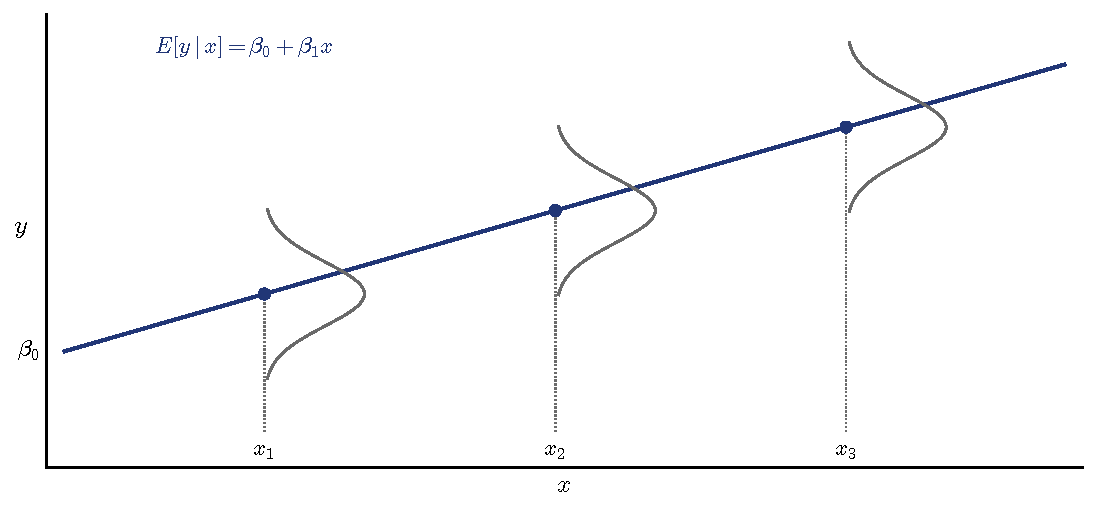
\includegraphics[width=.82\linewidth]{conditional_means.pdf}
\caption{Population conditional means at different $x$ values. Side curves indicate conditional distributions; this is a schematic illustration, not observed data.}
\label{fig:conditional-means}
\end{figure}
\paragraph{OLS: 普通最小二乘法.}
The \textbf{fitted} or sample regression line is
\begin{equation}\label{eq:fitted-simple}
\hat y_i=\hat\beta_0+\hat\beta_1x_i,
\qquad \hat\beta_0=\bar y-\hat\beta_1\bar x.
\end{equation}
For sample variation in $x$,
\begin{equation}\label{eq:simple-slope}
\hm{\hat\beta_1=
\frac{\sum_i(x_i-\bar x)(y_i-\bar y)}{\sum_i(x_i-\bar x)^2}
=\frac{\Cov_n(x,y)}{\Var_n(x)}
=r_{xy}\frac{s_y}{s_x}}.
\end{equation}
Here $r_{xy}=\Cov_n(x,y)/(s_xs_y)$. The numerator and denominator use the same covariance normalisation.\corr{slope-correlation}

\textbf{Slope.} Other factors being equal, a one-unit increase in $x$ is \hy{associated with} a \hy{predicted $\hat\beta_1$-unit increase} in $y$.
\blue{原稿例式：$y=\beta_0+\beta_1x+\beta_2z+\beta_3w+u$；若 $z,w$ 遗漏，简单回归系数可能把它们的影响一并算入。}

\red{相关不等于因果。}Without a justified data-generating process and identification assumptions, say ``associated with'' or ``correlated with'', rather than ``causes'', ``makes'' or ``leads to''. 若模型具有可辩护的结构性、外生性及因果识别条件，才可进一步解释为因果效应。\corr{causality}

\textbf{Intercept.} The fitted value of $y$ at $x=0$ is $\hat\beta_0$; under \eqref{eq:prf}, the population conditional mean at $x=0$ is $\beta_0$. This may be an extrapolation when $0$ is outside the observed or feasible range.

The fitted line depends on the sample; the population line is fixed but unknown. 原稿的 salary--roe 例式保留为
\[\widehat{\mathrm{salary}}=963.191+18.501\,\mathrm{roe}.\]
\begin{figure}[htbp]
\centering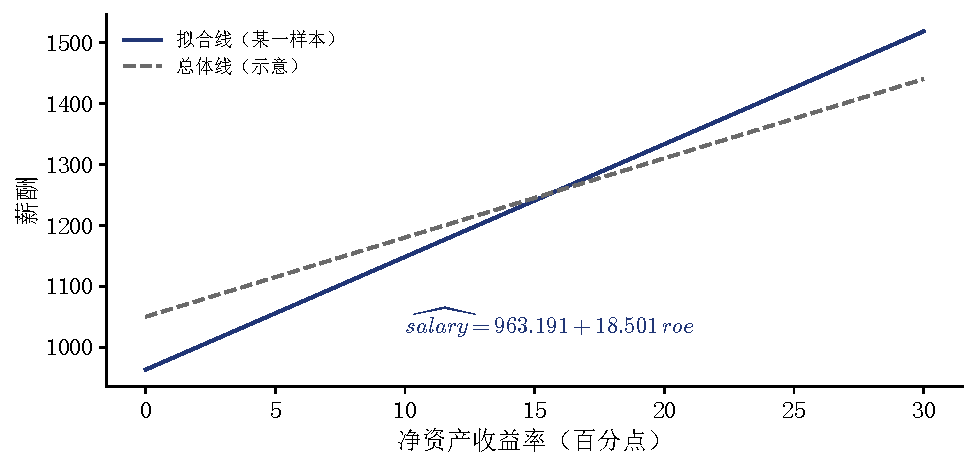
\includegraphics[width=.8\linewidth]{fitted_population.pdf}
\caption{Fitted versus population regression line, following the original salary--roe sketch. The population line is schematic, not an estimated benchmark.}
\label{fig:fitted-population}
\end{figure}

\subsection{Worked examples: units and percentage points}
\sourcepage{2}{3}{2/3}
\begin{example}[Hourly wage: 注意单位]\label{ex:wage-units}
The original specification measures hourly wage in \hy{thousands of dollars}, with education in years:
\[\wage=\beta_0+\beta_1\educ+u,\qquad
\widehat{\wage}=-0.9+0.54\educ.\]
Anson earns \$6 per hour and has 12 years of education. What would the model predict for him with 16 years, holding the unobserved component fixed?
\begin{align*}
\widehat{\wage}_{12}&=-0.9+0.54(12)=5.58\quad\text{(thousand dollars/hour)},\\
\hat u_{\rm Anson}&=0.006-5.58=-5.574,\\
\Delta\widehat{\wage}&=0.54(16-12)=2.16\quad\text{(thousand dollars/hour)},\\
\widehat{\wage}_{16}&=-0.9+0.54(16)=7.74.
\end{align*}
If the fitted residual is carried over unchanged in this model exercise,
\[\wage_{16}^{\rm scenario}=7.74-5.574=2.166,
\qquad\text{or }\$2{,}166\text{ per hour}.\]
Equivalently,
\[\hp{New scenario wage = old actual wage + modelled change},\]
\[\$6+(\$0.54\times10^3\times4)=\$2{,}166.\]
\added{The unusually large numbers follow the \emph{thousands} unit explicitly written in the source; they have not been silently changed to dollars. Keeping a person's error or fitted residual fixed is a hypothetical assumption, not an identified individual counterfactual or a guaranteed future actual wage.}\corr{wage-counterfactual}
\end{example}

\begin{exercise}[Election expenditure]\label{ex:election}
\[\widehat{\mathrm{voteA}}=26.81+0.464\,\mathrm{shareA}.\]
Here voteA is candidate A's vote percentage; shareA is A's percentage share of the two candidates' total campaign expenditure. A one-\hy{percentage-point} increase in shareA is associated with a 0.464-percentage-point increase in predicted voteA.
\begin{enumerate}
\item If shareA is $40\%$, enter $40$, not $0.40$:
\[\widehat{\mathrm{voteA}}=26.81+0.464(40)=\hm{45.37\%}.\]
If A spent nothing, the fitted value is $26.81$; if A accounted for all expenditure, it is $26.81+0.464(100)=73.21$. These are predictions from the fitted line, not election guarantees.
\item If candidate B spends 2 billion dollars, how much must A spend for the \emph{predicted} vote share to exceed $50\%$?
\begin{align*}
26.81+0.464\,\mathrm{shareA}&>50,\\
\mathrm{shareA}&>\frac{23.19}{0.464}=49.978448\ldots.
\end{align*}
\added{Let $A$ be expenditure in billions of dollars. Since $\mathrm{shareA}=100A/(A+2)$,
\[A>\frac{2(49.978448\ldots)}{100-49.978448\ldots}
=1.9982766\ldots\ \text{billion dollars}.\]
The strict inequality gives a threshold, not an attained minimum over continuous expenditure; actual victory cannot be guaranteed by this regression.}\corr{election}
\end{enumerate}
\end{exercise}

\section{Interpretation of Multiple OLS}
\sourcepage{2}{4}{2/4}
\label{sec:multiple-interpretation}
The population model and fitted line are
\begin{align}
y&=\beta_0+\beta_1x_1+\cdots+\beta_kx_k+u,\label{eq:multiple-model}\\
\hat y&=\hat\beta_0+\hat\beta_1x_1+\cdots+\hat\beta_kx_k.\label{eq:multiple-fitted}
\end{align}
For a fixed fitted equation,
\[\hm{\Delta\hat y=\hat\beta_1\Delta x_1+\cdots+\hat\beta_k\Delta x_k}.\]
Holding all the other $x_j$ fixed gives
\[\Delta\hat y=\hat\beta_\ell\Delta x_\ell,
\qquad\frac{\Delta\hat y}{\Delta x_\ell}=\hat\beta_\ell.
\]
\textbf{Partial effect.} In the population model, $\beta_\ell=\Delta y/\Delta x_\ell$ when all other regressors \emph{and} $u$ are held fixed; under ZCM it is also the partial slope of $\E[y\mid x_1,\ldots,x_k]$.\corr{notation}
\[\hy{$\E[u\mid x_1,\ldots,x_k]=0$}.\]
Including other explanatory variables permits their observed values to be held fixed in the fitted comparison. \blue{不需要 $x_\ell$ 与其他 $x_j$ 互不相关；只需避免完全共线性，才能区分各自系数。}

\begin{example}[College GPA]\label{ex:gpa}
\[\widehat{\colGPA}=1.29+0.453\hsGPA+0.0094\ACT.\]
The original ranges are colGPA: $0$--$4$; hsGPA: $1$--$4$; ACT (Achievement Test score): $0$--$36$.
\begin{description}
\item[hsGPA.] Holding ACT and all other factors fixed, another point in high-school GPA is associated with a predicted 0.453-point increase in college GPA.
\item[ACT.] Holding hsGPA and all other factors fixed, another point in ACT is associated with a predicted 0.0094-point increase in college GPA.
\item[Intercept.] The fitted college GPA at zero hsGPA and zero ACT is $1.29$. \red{Zero hsGPA is outside the stated range}, so this is an extrapolation, not the predicted GPA of an observed subgroup.
\end{description}
\begin{enumerate}
\item If hsGPA rises from $3.5$ to $3.6$ with ACT fixed,
\[\Delta\widehat{\colGPA}=(3.6-3.5)(0.453)=0.0453.\]
\item Anson has hsGPA $3.5$ and ACT $30$; Betty has hsGPA $3.0$ and ACT $36$:
\begin{align*}
\widehat{\colGPA}_{A}&=1.29+0.453(3.5)+0.0094(30)=3.1575,\\
\widehat{\colGPA}_{B}&=1.29+0.453(3.0)+0.0094(36)=2.9874.
\end{align*}
\item If Anson's actual GPA is $3.3$, can we infer Betty's actual GPA? No. \blue{每个人的 $u$ 不同，不能由一个人的实际值推出另一个人的实际值。} Anson's realised residual is $3.3-3.1575=0.1425$; Betty's residual is unknown.
\end{enumerate}
\end{example}


\section{Control Variables and the Frisch--Waugh--Lovell Theorem}
\sourcepage{2}{5}{2/5}
\label{sec:fwl-week2}
\subsection{Why introduce controls?}
Suppose the question is the effect of education $x_1$ on wages $y$, and ability $x_2$ also matters:
\[y=\beta_0+\beta_1x_1+\beta_2x_2+u.\]
If ability is omitted, the short equation $y=\tilde\beta_0+\tilde\beta_1x_1+v$ may attribute ability's influence to education. This is \hp{omitted variable bias}（遗漏变量偏误）when ability both affects wages and is associated with education.

There are two interpretations of controlling:
\begin{enumerate}
\item \hy{Holding constant}: compare changes in $x_1$ while holding $x_2$ fixed.
\item \hy{Partialling out}: remove the linear component explained by $x_2$ before reading the coefficient on $x_1$.
\end{enumerate}
\blue{二者描述的是同一个多元回归系数；FWL 将“排除其他变量的线性影响”写成可计算的步骤。}

\subsection{Residualising the regressor}
In the sample, first regress $x_1$ on a constant and $x_2$:
\begin{equation}\label{eq:fwl-x}
x_{1i}=\hat\delta_0+\hat\delta_1x_{2i}+\hat r_{1i}.
\end{equation}
The residual $\hat r_{1i}$ is the part of $x_{1i}$ \hy{not linearly explained by $x_2$}; it satisfies
\[\sum_i\hat r_{1i}=0,\qquad\sum_i x_{2i}\hat r_{1i}=0.\]
Regress $y_i$ on a constant and $\hat r_{1i}$. Its slope is exactly the coefficient on $x_1$ in the original multiple OLS regression:
\begin{equation}\label{eq:fwl-one-sided}
\hm{\hat\beta_1=
\frac{\Cov_n(\hat r_1,y)}{\Var_n(\hat r_1)}
=\frac{\sum_i\hat r_{1i}y_i}{\sum_i\hat r_{1i}^2}}.
\end{equation}
Thus $\hat\beta_1$ measures the fitted relationship between $y$ and the variation in $x_1$ left after removing its linear relationship with $x_2$. \blue{将 $x_1$ 对控制变量回归，留下不被它们线性解释的部分。}

\added{For the standard two-sided FWL regression, also regress $y$ on $(1,x_2)$ and obtain $\hat r_{yi}$. Regress $\hat r_y$ on $\hat r_1$ without an intercept. This gives the same slope \emph{and the same residuals} as the full model. The one-sided regression in the original note gives the same slope, but generally not the same regression residuals.}\corr{fwl-residual}

\subsection{General case}
For $y=\beta_0+\beta_1x_1+\cdots+\beta_kx_k+u$, regress $x_1$ on $(1,x_2,\ldots,x_k)$:
\[x_{1i}=\hat\delta_0+\hat\delta_2x_{2i}+\cdots+\hat\delta_kx_{ki}+\hat r_{1i}.\]
Regress $y_i$ on $\hat r_{1i}$ and a constant, or regress the correspondingly residualised $y_i$ on $\hat r_{1i}$ without a constant. Formula \eqref{eq:fwl-one-sided} still holds when the residual variation is positive. More details and the repeated derivation are retained in \hyperref[sec:fwl-week3]{Week 3} and \hyperref[sec:fwl-week4]{Week 4}.

\section{Simple versus Multiple Regression Slopes}
\sourcepage{2}{6}{2/6}
\label{sec:short-long-week2}
If a control is added, must it be uncorrelated with the original regressor? \red{不用！} Correlated controls are precisely why simple and multiple slopes often differ. A control must, however, be appropriate to the causal or predictive question; adding it does not automatically remove bias.

Consider the population equations
\begin{align*}
y&=\beta_0+\beta_1x_1+\beta_2x_2+u,\\
x_2&=\delta_0+\delta_1x_1+\varepsilon.
\end{align*}
The second equation is a population linear projection, with $\E[\varepsilon]=\E[x_1\varepsilon]=0$. If $\E[u\mid x_1,x_2]=0$, substitution gives
\begin{align*}
y&=\beta_0+\beta_1x_1+\beta_2(\delta_0+\delta_1x_1+\varepsilon)+u\\
 &=\underbrace{(\beta_0+\beta_2\delta_0)}_{\tilde\beta_0}
  +\underbrace{(\beta_1+\beta_2\delta_1)}_{\tilde\beta_1}x_1
  +\underbrace{(u+\beta_2\varepsilon)}_{v}.
\end{align*}
Hence the short population projection slope is
\begin{equation}\label{eq:population-ovb}
\hm{\tilde\beta_1=\beta_1+\beta_2\delta_1}.
\end{equation}
This is a relation between \emph{population projection coefficients}, not an equality between an estimator and a fixed parameter.\corr{ovb-levels}

\paragraph{When do the slopes coincide?}
For the two-regressor case, $\tilde\beta_1=\beta_1$ exactly when $\beta_2\delta_1=0$:
\begin{enumerate}
\item $\beta_2=0$: the partial effect of $x_2$ on $y$ is zero; the population slopes coincide even if $x_1$ and $x_2$ are correlated.
\item $\delta_1=0$: $x_1$ and $x_2$ are uncorrelated in the population.
\end{enumerate}
\added{For realised OLS coefficients, the exact sample identity is
\[\hat{\tilde\beta}_1=\hat\beta_1+\hat\beta_2\hat\delta_1.\]
Sample slopes therefore coincide if $\hat\beta_2=0$ or the \emph{sample} auxiliary slope $\hat\delta_1=0$. A zero population coefficient does not force its sample estimate to be exactly zero.}

\begin{example}[GPA: controls change the interpretation]\label{ex:gpa-short-long}
Compare the following rounded fitted equations:
\begin{align*}
\widehat{\colGPA}&=1.29+0.453\hsGPA+0.0094\ACT,\\
\widehat{\colGPA}&\simeq2.40+0.0271\ACT
                       &&\text{(ACT only)},\\
\widehat{\hsGPA}&\simeq2.46+0.039\ACT,\\
\widehat{\colGPA}&\simeq1.41+0.482\hsGPA
                       &&\text{(hsGPA only)}.
\end{align*}
For ACT, the population/sample substitution intuition is visible in the rounded arithmetic:
\[1.29+0.453(2.46)=2.40438,\qquad
0.0094+0.453(0.039)=0.027067\simeq0.0271.\]
The hsGPA-only slope is fairly close to its multiple-regression slope, in part because the partial ACT coefficient is small. \blue{小的遗漏系数只有与辅助回归系数的大小一起看，才说明偏差是否小。} All displayed regressions are the source's rounded examples, not newly estimated empirical results.
\end{example}

\section{Units and Functional Form}
\sourcepage{2}{7}{2/7}
\label{sec:units}
\subsection{Changing the unit of the dependent variable}
Start from $y=\beta_0+\beta_1x+u$. For $y'=cy$ with $c\ne0$,
\[y'=c\beta_0+c\beta_1x+cu.\]
Therefore
\[\hy{$\beta'_0=c\beta_0$},\qquad
\hy{$\beta'_1=c\beta_1$},\qquad u'=cu,\qquad\Delta y'=c\Delta y.\]
For example, converting dollars into thousands of dollars uses $c=1/1000$.
The sample OLS derivation is
\begin{align*}
\hat\beta'_1
 &=\frac{\Cov_n(x,y')}{\Var_n(x)}
 =\frac{\Cov_n(x,cy)}{\Var_n(x)}
 =c\hat\beta_1,\\
\hat\beta'_0
 &=\bar y'-\hat\beta'_1\bar x
 =c\bar y-c\hat\beta_1\bar x=c\hat\beta_0.
\end{align*}
Under ZCM, the intercept interpretation at $x=0$ becomes
\[\E[y'\mid x=0]=c\beta_0=\beta'_0.\]
\red{这里必须写条件均值；通常不能写成 $\beta_0=\E[y]$。} In general $\E[y]=\beta_0+\beta_1\E[x]$ when $\E[u]=0$.\corr{unit-intercept}

\subsection{Changing the unit of the regressor}
If $x'=cx$ with $c\ne0$, then
\[y=\beta_0+\frac{\beta_1}{c}x'+u,\qquad
\hy{$\beta'_0=\beta_0$},\quad\hy{$\beta'_1=\beta_1/c$}.\]
At $x'=0$ we also have $x=0$, so the intercept is unchanged. For the fitted coefficients,
\begin{align*}
\hat\beta'_1
 &=\frac{\Cov_n(x',y)}{\Var_n(x')}
 =\frac{c\Cov_n(x,y)}{c^2\Var_n(x)}
 =\frac{\hat\beta_1}{c},\\
\hat\beta'_0&=\bar y-\frac{\hat\beta_1}{c}(c\bar x)=\hat\beta_0.
\end{align*}
The fitted mean identity is correspondingly $\bar y=\hat\beta'_0+\hat\beta'_1\bar x'$.

\section{Level and Log Specifications}
\sourcepage{2}{8}{last page}
\label{sec:logs}
\blue{Level 对应单位变化；log 对应相对或百分比变化。} All logs below are natural logs; logarithms require positive arguments. Throughout the comparison, the error and other regressors are held fixed. Write $\%\Delta x=100\Delta x/x_0$ and $\%\Delta y=100\Delta y/y_0$ for ordinary finite percentage changes.

\subsection{Level--level}
\[y=\beta_0+\beta_1x+u,\qquad
\hm{\Delta y=\beta_1\Delta x}.\]
One unit more in $x$ corresponds to $\beta_1$ units more in $y$.

\subsection{Level--log}
\[y=\beta_0+\beta_1\ln x+u,\qquad
\frac{dy}{d\ln x}=\beta_1,\qquad
dy=\beta_1\frac{dx}{x}.\]
For a small change,
\[\hm{\Delta y\approx\frac{\beta_1}{100}\,\%\Delta x}.\]
A one-percent increase in $x$ is associated with approximately $\beta_1/100$ units more in $y$.
\added{For a finite change, the exact model relation is $\Delta y=\beta_1\ln(x_1/x_0)$. For a 1\% increase it is $\beta_1\ln(1.01)$, not exactly $\beta_1/100$.}\corr{logs}

\subsection{Log--level}
\[\ln y=\beta_0+\beta_1x+u,\qquad
\frac{d\ln y}{dx}=\beta_1=\frac{1}{y}\frac{dy}{dx}.\]
Thus $\beta_1$ is a semi-elasticity, stored as a decimal, and
\[\hm{\%\Delta y\approx100\beta_1\Delta x}.\]
One unit more in $x$ corresponds to approximately $100\beta_1$ percent more in $y$.
\added{For finite $\Delta x$, the exact constant-error relation is
\[\%\Delta y=100\bigl(e^{\beta_1\Delta x}-1\bigr).\]
Exponentiating $\E[\ln y\mid x]$ is not generally the same as $\E[y\mid x]$; a statement about the mean in levels requires a retransformation adjustment.}\corr{logs}

\subsection{Log--log}
\[\ln y=\beta_0+\beta_1\ln x+u,\qquad
\hm{\beta_1=\frac{d\ln y}{d\ln x}
=\frac{dy/y}{dx/x}}.\]
$\beta_1$ is the elasticity. For small changes,
\[\%\Delta y\approx\beta_1\,\%\Delta x.\]
One percent more in $x$ corresponds to approximately $\beta_1$ percent more in $y$.
\added{For an ordinary finite percentage change $p=\%\Delta x$,
\[\%\Delta y=100\left[\left(1+\frac p{100}\right)^{\beta_1}-1\right].\]
The differential elasticity is exact; replacing differentials with arbitrary finite changes is an approximation.}\corr{logs}

\subsection*{Chapter recap / 本章小结}
\addcontentsline{toc}{subsection}{Chapter recap / 本章小结}
\begin{itemize}
\item A fitted slope is a predicted association; a causal interpretation needs an appropriate model and research design.
\item Multiple OLS holds included controls fixed; FWL isolates the same slope through residualisation.
\item Units rescale coefficients. Log specifications require clear separation of exact relations and percentage approximations.
\end{itemize}

\chapter{Goodness of Fit}
\label{ch:week3}
\section{The Simple Regression Case}
\sourcepage{3}{1}{3/1}
\label{sec:simple-properties}
This chapter separates fitted values from residuals and develops the coefficient of determination $R^2$.
\[y_i=\beta_0+\beta_1x_i+u_i,\qquad
\hat y_i=\hat\beta_0+\hat\beta_1x_i.\]
\begin{definition}[Error and residual]
\[\underbrace{u_i=y_i-\beta_0-\beta_1x_i}_{\text{population error}},\qquad
\underbrace{\hat u_i=y_i-\hat y_i=y_i-\hat\beta_0-\hat\beta_1x_i}_{\text{OLS residual}}.\]
The residual is observable after fitting; the error depends on unknown population parameters.
\end{definition}

\subsection{Three sample properties of OLS with an intercept}
\paragraph{Property 1: residuals have sample mean zero.}
OLS minimises $Q(b_0,b_1)=\sum_i(y_i-b_0-b_1x_i)^2$. At the optimum,
\[\left.\frac{\partial Q}{\partial b_0}\right|_{\hat\beta}
=-2\sum_{i=1}^n\hat u_i=0
\quad\Longrightarrow\quad\hm{\sum_i\hat u_i=0},\quad\bar{\hat u}=0.\]

\paragraph{Property 2: residuals are sample-orthogonal to $x$.}
The slope first-order condition is
\[\left.\frac{\partial Q}{\partial b_1}\right|_{\hat\beta}
=-2\sum_i x_i\hat u_i=0.\]
Consequently,
\begin{align*}
\Cov_n(x,\hat u)
&=\frac1n\sum_i(x_i-\bar x)(\hat u_i-\bar{\hat u})\\
&=\frac1n\left(\sum_i x_i\hat u_i-\bar x\sum_i\hat u_i\right)=0.
\end{align*}
\hy{Residuals are uncorrelated with $x$ in the sample}. Correlation itself is undefined if a variance is zero; orthogonality remains a valid statement.

Each observation decomposes into $y_i=\hat y_i+\hat u_i$, with fitted values and residuals sample-orthogonal:
\[\sum_i\hat y_i\hat u_i
=\hat\beta_0\sum_i\hat u_i+\hat\beta_1\sum_i x_i\hat u_i=0.\]

\paragraph{Population moments: a separate statement.}
The population moments can be obtained using the law of iterated expectations. Under $\E[u\mid x]=0$ and the required integrability,
\[\E[u]=\E\{\E[u\mid x]\}=0,\qquad
\E[xu]=\E\{x\E[u\mid x]\}=0.\]
\red{These population restrictions do not prove the sample normal equations.} The sample identities above follow mechanically from minimising squared residuals, even if the population exogeneity assumption is false.\corr{sample-population}

\paragraph{Property 3: the sample mean lies on the fitted line.}
Since $\hat\beta_0=\bar y-\hat\beta_1\bar x$,
\[\hm{\bar y=\hat\beta_0+\hat\beta_1\bar x}.\]
Alternatively, average $\hat y_i=\hat\beta_0+\hat\beta_1x_i$:
\[\bar{\hat y}=\frac1n\sum_i\hat y_i=\hat\beta_0+\hat\beta_1\bar x,
\qquad\bar y=\bar{\hat y}+\bar{\hat u}=\bar{\hat y}.\]
The \emph{population} counterpart is $\E[y]=\beta_0+\beta_1\E[x]$ if $\E[u]=0$; it uses population coefficients, not fitted hats.\corr{sample-population}

\section{Sums of Squares and Goodness of Fit}
\sourcepage{3}{2}{3/2}
\label{sec:ss-decomposition}
\begin{definition}[TSS, ESS and RSS]
\begin{align}
\TSS&=\sum_{i=1}^n(y_i-\bar y)^2=(n-1)s_y^2,\label{eq:tss}\\
\ESS&=\sum_{i=1}^n(\hat y_i-\bar y)^2,\label{eq:ess}\\
\RSS&=\sum_{i=1}^n\hat u_i^2=\sum_{i=1}^n(y_i-\hat y_i)^2.\label{eq:rss}
\end{align}
Here $s_y^2=\sum_i(y_i-\bar y)^2/(n-1)$ is the sample variance.
\end{definition}
\blue{TSS：$y$ 围绕均值的总波动；ESS：回归线所解释的波动；RSS：回归未解释的残差波动。} Here ESS means \emph{explained} sum of squares; other books sometimes use different abbreviations.

\begin{theorem}[Sum-of-squares decomposition]
For OLS with an intercept,
\begin{equation}\label{eq:anova}
\hm{\TSS=\ESS+\RSS}.
\end{equation}
\end{theorem}
\begin{proof}
Since $y_i-\bar y=(\hat y_i-\bar y)+\hat u_i$,
\begin{align*}
\TSS
&=\sum_i\bigl[(\hat y_i-\bar y)+\hat u_i\bigr]^2\\
&=\sum_i(\hat y_i-\bar y)^2+\sum_i\hat u_i^2
  +2\sum_i\hat u_i(\hat y_i-\bar y).
\end{align*}
The cross-term is zero because $\sum_i\hat u_i\hat y_i=0$ and $\sum_i\hat u_i=0$. Hence \eqref{eq:anova} follows.
\end{proof}
\blue{OLS 的目标是使 $\sum_i\hat u_i^2$ 最小，而不是使 $\sum_i\hat u_i$ 最小；后者为零来自截距的一阶条件。}

\subsection[Definition and interpretation of R-squared]{Definition and interpretation of $R^2$}
For $\TSS>0$, define
\begin{equation}\label{eq:r2}
\hm{R^2=\frac{\ESS}{\TSS}=1-\frac{\RSS}{\TSS}\in[0,1]}.
\end{equation}
\textbf{Interpretation.} $R^2$ measures the \hy{proportion of sample variation in $y$} explained by the fitted regressors. For example, $R^2=0.85$ means $85\%$ of the sample variation in the dependent variable is explained by the regression.

If every point lies on the fitted line, $y_i=\hat y_i$, then $\RSS=0$, $\TSS=\ESS$, and $R^2=1$. This is the perfect-fit case.
\begin{figure}[htbp]
\centering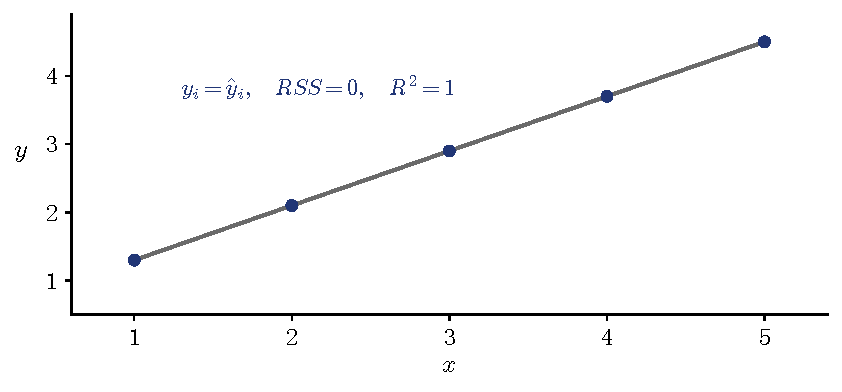
\includegraphics[width=.68\linewidth]{perfect_fit.pdf}
\caption{The source's perfect-fit case: all schematic observations lie on the fitted line.}
\label{fig:perfect-fit}
\end{figure}

\subsection{Squared correlation interpretation}
When $y$ and $\hat y$ both have positive sample variance,
\begin{equation}\label{eq:r2-correlation}
R^2=\Corr_n(y,\hat y)^2
=\frac{\left[\sum_i(y_i-\bar y)(\hat y_i-\bar y)\right]^2}
{\left[\sum_i(y_i-\bar y)^2\right]\left[\sum_i(\hat y_i-\bar y)^2\right]}.
\end{equation}
To see this, use $y_i=\hat y_i+\hat u_i$, $\bar y=\bar{\hat y}$ and sample orthogonality:
\[\Cov_n(y,\hat y)=\Var_n(\hat y),\qquad
\Corr_n(y,\hat y)^2=\frac{\Var_n(\hat y)}{\Var_n(y)}=\frac{\ESS}{\TSS}.
\]
\added{If all $y_i$ are equal, TSS is zero and this centred $R^2$ is undefined. If $\hat y$ is constant while $y$ varies, $R^2=0$ but $\Corr_n(y,\hat y)$ is undefined; the squared-correlation formula then cannot be evaluated.}\corr{r2-degenerate}

\subsection{Graphical comparison}
\sourcepage{3}{3}{3/3}
\begin{figure}[htbp]
\centering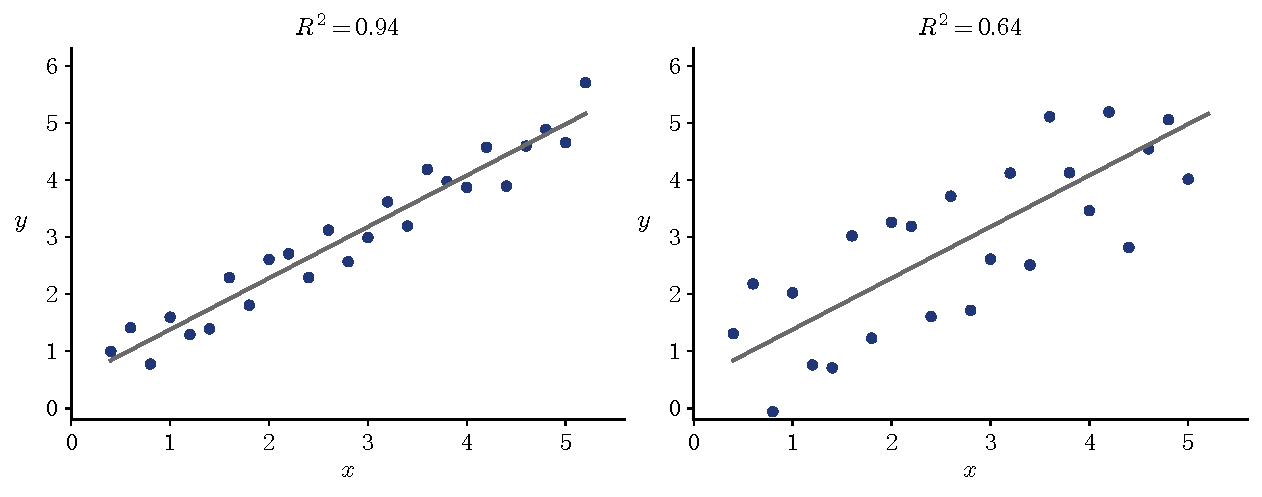
\includegraphics[width=.95\linewidth]{r_squared_comparison.pdf}
\caption{Schematic samples with the source's $R^2=0.94$ and $R^2=0.64$. The labels are computed from the generated points and fitted lines.}
\label{fig:r2-comparison}
\end{figure}
High $R^2$ corresponds to a smaller residual \emph{share} $\RSS/\TSS$; low $R^2$ corresponds to a larger residual share. \blue{仅靠当前回归变量，对 $y$ 的样本波动解释得较少。} Comparing absolute RSS across different samples or differently scaled outcomes is not justified by $R^2$ alone.\corr{r2-rss}

\section{The Multiple Regression Case}
\label{sec:multiple-properties}
The model, fitted values and residuals are
\begin{align*}
y_i&=\beta_0+\beta_1x_{1i}+\cdots+\beta_kx_{ki}+u_i,\\
\hat y_i&=\hat\beta_0+\hat\beta_1x_{1i}+\cdots+\hat\beta_kx_{ki},\\
\hat u_i&=y_i-\hat y_i.
\end{align*}
The three sample properties extend to multiple regression as follows.

\paragraph{Property 1: residuals have mean zero.}
With $Q(b)=\sum_i(y_i-b_0-\sum_{j=1}^k b_jx_{ji})^2$,
\[\left.\frac{\partial Q}{\partial b_0}\right|_{\hat\beta}
=-2\sum_i\hat u_i=0
\quad\Longrightarrow\quad\sum_i\hat u_i=0,\quad\bar{\hat u}=0.\]

\paragraph{Property 2: residuals are sample-orthogonal to every included regressor.}
For each $j=1,\ldots,k$,
\[\left.\frac{\partial Q}{\partial b_j}\right|_{\hat\beta}
=-2\sum_i x_{ji}\hat u_i=0
\quad\Longrightarrow\quad\hm{\sum_i x_{ji}\hat u_i=0}.\]
Together with the intercept condition, this gives $\Cov_n(x_j,\hat u)=0$.

\paragraph{Property 3: the vector of sample means lies on the fitted hyperplane.}
Averaging $y_i=\hat y_i+\hat u_i$ gives $\bar y=\bar{\hat y}$. Hence
\begin{align*}
\bar y
&=\frac1n\sum_i\left(\hat\beta_0+\hat\beta_1x_{1i}+\cdots+\hat\beta_kx_{ki}\right)\\
&=\hm{\hat\beta_0+\hat\beta_1\bar x_1+\cdots+\hat\beta_k\bar x_k}.
\end{align*}
The same proof of \eqref{eq:anova} gives TSS $=$ ESS $+$ RSS and the same formula for $R^2$ in multiple OLS with an intercept.

\section[Adding Regressors and Adjusted R-squared]{Adding Regressors and Adjusted $R^2$}
\sourcepage{3}{4}{3/4}
\label{sec:adjusted-r2}
Recall
\[\TSS=\sum_i(y_i-\bar y)^2,\quad
\ESS=\sum_i(\hat y_i-\bar y)^2,\quad
\RSS=\sum_i(y_i-\hat y_i)^2.\]
What happens to $R^2$ if more regressors are added?
\begin{itemize}
\item With the \emph{same observations and outcome}, and an intercept in both nested models, the new least-squares RSS cannot exceed the old RSS: the old fit remains available by setting the new coefficients to zero.
\item Thus $R^2$ \hy{cannot decrease}; it may stay exactly unchanged. Repeatedly adding variables can overfit the sample.\corr{r2-monotonic}
\item $R^2$ does not establish a causal relationship. A high $R^2$ need not mean causation, and a low $R^2$ does not rule it out.
\end{itemize}

\subsection{Degrees-of-freedom adjustment}
For $k$ regressors excluding the intercept, $n>k+1$ and $\TSS>0$,
\begin{equation}\label{eq:adjusted-r2}
\hm{\bar R^2=1-\frac{\RSS/(n-k-1)}{\TSS/(n-1)}
=1-\frac{n-1}{n-k-1}(1-R^2)}.
\end{equation}
\blue{自由度修正：增加回归变量会受到惩罚，RSS 的减少必须足以补偿损失的自由度。}
\begin{itemize}
\item $\bar R^2$ penalises the number of regressors; it can decrease when another regressor is added.
\item It can be negative when the residual mean square exceeds the mean-only baseline mean square.
\item A rise in $\bar R^2$ means a sufficient in-sample fit improvement under this adjustment, not proof of substantive importance or causality.
\end{itemize}
\added{For $q$ added regressors, $\bar R^2$ rises precisely when
\[
\frac{(\RSS_{\rm old}-\RSS_{\rm new})/q}{\RSS_{\rm new}/(n-k_{\rm new}-1)}>1,
\]
assuming a positive denominator. This is a descriptive partial-$F$ threshold of 1, not a conventional significance cutoff.}\corr{adjusted-meaning}

\begin{example}[GPA: the trade-off in the original note]
Using the displayed rounded values and $n=141$:
\begin{align*}
\text{hsGPA only: }\quad &R^2=0.172,\quad k=1,\\
&\bar R^2=1-\frac{140}{139}(1-0.172)=0.166043\ldots,\\
\text{hsGPA and ACT: }\quad &R^2=0.176,\quad k=2,\\
&\bar R^2=1-\frac{140}{138}(1-0.176)=0.164058\ldots.
\end{align*}
Adding ACT raises ordinary $R^2$, while adjusted $R^2$ falls slightly. These values are computed from the source's rounded inputs, so precision beyond the shown inputs is only arithmetic precision.
\end{example}

\paragraph{注意（保留原稿的三点提醒）.}
\begin{enumerate}
\item $R^2$ describes sample fit: 高 $R^2\ne$ 因果，低 $R^2\ne$ 没有因果。
\item Adding variables can overfit; adjusted $R^2$ supplies a penalty, but does not by itself certify out-of-sample performance.
\item A good fit does not automatically eliminate omitted-variable bias.
\end{enumerate}


\section{Regression through the Origin and Demeaning}
\sourcepage{3}{5}{3/5}
\label{sec:rto}
Recall $\hat\beta_0=\bar y$ for an \emph{intercept-only} regression; the proof appears below. This identity does not apply to an arbitrary regression containing $x$.

\subsection{Regression through the origin (RTO)}
Sometimes a model is restricted to pass through the origin, for example a production relation in which zero input is assumed to imply zero expected output. This is an additional modelling restriction, not an automatic property of production data.
\[y_i=\beta_1^{\rm RTO}x_i+u_i,\qquad
\hat y_i=\check\beta_1x_i,\qquad\check u_i=y_i-\hat y_i.\]
Use a check accent here to distinguish this fitted slope and its residual from OLS with an intercept. Minimising
\[Q(b_1)=\sum_i(y_i-b_1x_i)^2\]
gives the first-order condition
\[\sum_i x_i(y_i-\check\beta_1x_i)=0
\quad\Longrightarrow\quad
\hm{\check\beta_1=\frac{\sum_i x_iy_i}{\sum_i x_i^2}}
\quad\text{if }\sum_i x_i^2>0.
\]

\subsection{Demeaned variables reproduce the slope with an intercept}
Define $A_i=y_i-\bar y$ and $B_i=x_i-\bar x$. A through-origin regression of $A_i$ on $B_i$ has slope
\[\frac{\sum_iB_iA_i}{\sum_iB_i^2}
=\frac{\sum_i(x_i-\bar x)(y_i-\bar y)}{\sum_i(x_i-\bar x)^2}
=\hat\beta_1.\]
Thus a no-intercept regression of \emph{demeaned} variables reproduces the slope in ordinary OLS \emph{with} an intercept. It does not mean an uncentred no-intercept regression gives the same slope.\corr{demeaning}

For OLS with an intercept,
\[y_i-\bar y=\hat\beta_1(x_i-\bar x)+\hat u_i.\]
\blue{截距项使回归线经过样本均值 $(\bar x,\bar y)$；去均值相当于平移坐标，不改变斜率。}
\begin{figure}[htbp]
\centering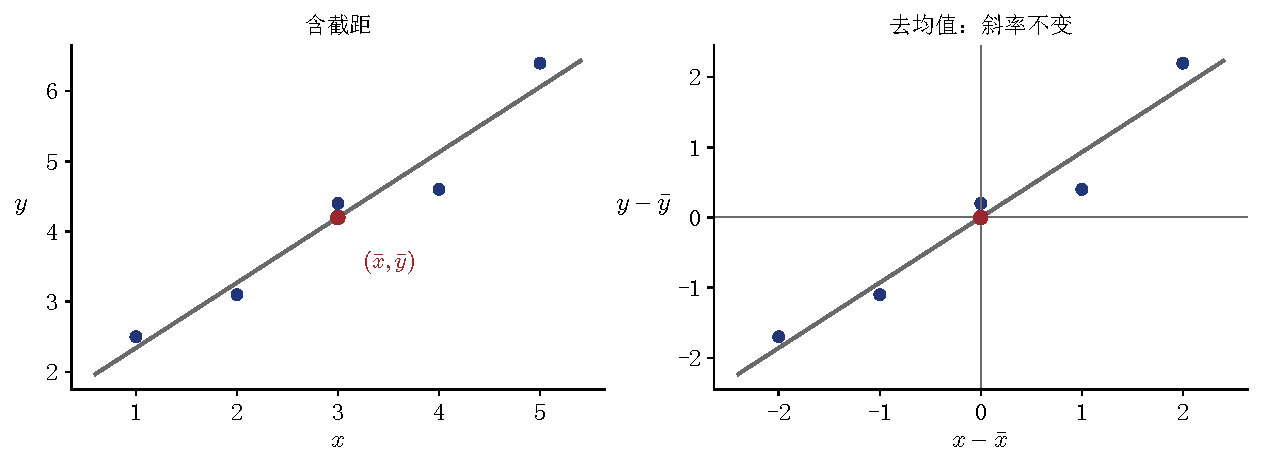
\includegraphics[width=.95\linewidth]{demeaning.pdf}
\caption{Demeaning shifts the sample mean to the origin and preserves the fitted slope. Schematic observations.}
\label{fig:demeaning}
\end{figure}

\paragraph{原稿页底重复的例式（保留可见内容）.}
The scan ends with the repeated example
\[\wage=\beta_0+\beta_1\educ+u,\]
and the list of unobservable factors: intelligence, family background, experience, training, etc. These factors are again relevant to the exogeneity discussion in Week 2. No continuation beyond the visible scan is inferred.

\subsection{OLS formulas, repeated as in the supplementary sheet}
\sourcepage{3}{6}{supplementary derivation sheet}
With an intercept,
\[\hat\beta_1=\frac{\sum_i(x_i-\bar x)(y_i-\bar y)}{\sum_i(x_i-\bar x)^2},
\qquad\hat\beta_0=\bar y-\hat\beta_1\bar x.\]
Without an intercept,
\begin{align*}
\frac{d}{db_1}\sum_i(y_i-b_1x_i)^2&=-2\sum_i x_i(y_i-b_1x_i),\\
\sum_i x_iy_i-\check\beta_1\sum_i x_i^2&=0,\\
\check\beta_1&=\frac{\sum_i x_iy_i}{\sum_i x_i^2}.
\end{align*}

\paragraph{Why does demeaning work? 去均值.}
Let $x_i^*=x_i-\bar x$ and $y_i^*=y_i-\bar y$. Regress $y_i^*$ on $x_i^*$ without an intercept:
\[\hat\gamma=\frac{\sum_i x_i^*y_i^*}{\sum_i(x_i^*)^2}
=\frac{\sum_i(x_i-\bar x)(y_i-\bar y)}{\sum_i(x_i-\bar x)^2}=\hat\beta_1.\]
Hence: OLS with an intercept $\Longleftrightarrow$ demeaned OLS without an intercept, for the slope. The sample-mean point becomes $(0,0)$ without rotating the fitted line.

\paragraph{Demeaning is regression on a constant.}
In an intercept-only regression $y_i=b_0+e_i$,
\[\frac{d}{db_0}\sum_i(y_i-b_0)^2=-2\sum_i(y_i-b_0)=0
\quad\Longrightarrow\quad\hat b_0=\bar y.\]
Its residual is $y_i-\bar y$. Likewise, regressing $x_i$ on a constant yields residual $x_i-\bar x$.

\subsection{Partialling out: the FWL theorem}
\label{sec:fwl-week3}
For $y_i=\beta_0+\beta_1x_i+\beta_2z_i+u_i$, the source's three-step recipe is:
\begin{enumerate}
\item Regress $y$ on $(1,z)$ and obtain residuals $r_{yi}$.
\item Regress $x$ on $(1,z)$ and obtain residuals $r_{xi}$.
\item Regress $r_y$ on $r_x$ without an intercept.
\end{enumerate}
The result is
\[\hm{\hat\beta_1=\frac{\sum_i r_{xi}r_{yi}}{\sum_i r_{xi}^2}}.\]
Demeaning is the special case where the only variable being partialled out is a constant. This retains the source's connection between the two procedures.

\section{OLS Properties without an Intercept}
\sourcepage{3}{7}{3/6}
\label{sec:rto-properties}
Return to the RTO objective and its only coefficient first-order condition:
\[\min_{b_1}\sum_i(y_i-b_1x_i)^2,\qquad
-2\sum_i x_i(y_i-\check\beta_1x_i)=0
\quad\Longrightarrow\quad\sum_i x_i\check u_i=0.\]
There is no intercept coefficient with respect to which to differentiate.

\paragraph{Property 1: mean-zero residuals need not hold.}
The condition $\sum_i\check u_i=0$ is no longer imposed; it can hold in special samples, but is not guaranteed.

\paragraph{Property 2: orthogonality survives, covariance need not.}
We still have $\sum_i x_i\check u_i=0$. However,
\[\Cov_n(x,\check u)=\frac1n\sum_i x_i\check u_i-\bar x\bar{\check u}
=-\bar x\bar{\check u},\]
which is generally nonzero. \red{不能在无截距时把“内积为零”直接写成“样本不相关”。}\corr{rto-covariance}

\paragraph{Property 3: the sample mean need not lie on the line.}
Averaging $y_i=\check\beta_1x_i+\check u_i$ gives
\[\bar y=\check\beta_1\bar x+\bar{\check u}.\]
Thus $\bar y=\check\beta_1\bar x$ is not generally true. With an intercept, by contrast, $\bar{\hat u}=0$ implies $\bar y=\bar{\hat y}$.

\subsection[Centred R-squared may be negative]{Centred $R^2$ may be negative}
Using the same centred definitions of TSS and ESS,
\begin{equation}\label{eq:rto-cross-term}
\TSS=\ESS+\RSS+2\sum_i\check u_i(\hat y_i-\bar y).
\end{equation}
For a through-origin fit, $\sum_i\check u_i\hat y_i=0$ but $\sum_i\check u_i$ need not vanish. Consequently the cross-term need not be zero.\corr{rto-cross-term}
The centred statistic
\[R_c^2=1-\frac{\RSS}{\TSS}\]
can be negative: the forced-through-origin line then fits worse in squared-error terms than the horizontal mean-only line $\bar y$.
\begin{figure}[htbp]
\centering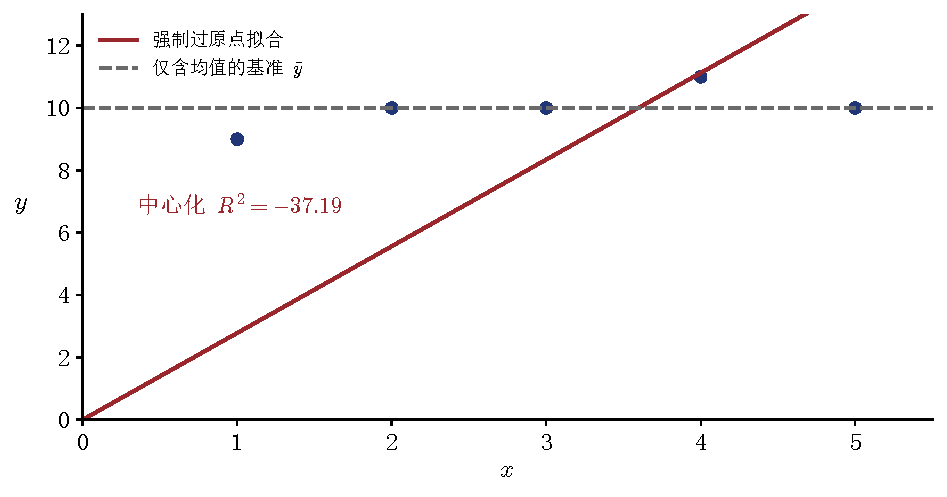
\includegraphics[width=.8\linewidth]{through_origin_negative_r2.pdf}
\caption{A through-origin fit worse than the mean-only baseline. Schematic data $x=(1,2,3,4,5)$, $y=(9,10,10,11,10)$ produce the negative centred $R^2$ computed in the figure.}
\label{fig:negative-r2}
\end{figure}
\added{Some software reports an \emph{uncentred} statistic $R_u^2=1-\RSS/\sum_i y_i^2$ for a model without an intercept. Its baseline is zero rather than $\bar y$, so it is not directly comparable with the usual centred $R^2$ of a model with an intercept.}\corr{rto-r2}

\subsection*{Chapter recap / 本章小结}
\addcontentsline{toc}{subsection}{Chapter recap / 本章小结}
\begin{itemize}
\item With an intercept, OLS residuals have zero mean, are sample-orthogonal to included regressors, and yield TSS $=$ ESS $+$ RSS.
\item Ordinary $R^2$ cannot fall when regressors are added to a nested model on the same data; adjusted $R^2$ can fall.
\item Demeaning and FWL preserve the relevant full-model slope. Omitting the intercept changes the mean, covariance and centred-$R^2$ properties.
\end{itemize}

\chapter{Unbiasedness of OLS Estimation}
\label{ch:week4}
\section{Concept, Assumptions and Theorem: Simple OLS}
\sourcepage{4}{1}{4/1}
\label{sec:unbiasedness-concept}
Objectives:
\begin{enumerate}
\item State the assumptions for \hy{finite-sample unbiasedness}（有限样本无偏性）.
\item Explain zero conditional mean in economic language（用经济语言解释零条件均值）.
\item Determine the direction of omitted-variable bias in standard cases.
\end{enumerate}
\subsection{Recap of estimation and goodness of fit}
\[y=\beta_0+\beta_1x+u,\qquad
\hat y=\hat\beta_0+\hat\beta_1x,\]
\[\hat\beta_1=\frac{\Cov_n(x,y)}{\Var_n(x)},\qquad
\hat\beta_0=\bar y-\hat\beta_1\bar x,\qquad
R^2=\frac{\ESS}{\TSS}=1-\frac{\RSS}{\TSS}.\]
The $R^2$ identity here assumes an intercept and positive TSS.

\subsection{A parameter versus an estimator}
\begin{description}
\item[$\beta_j$.] A fixed but unknown population parameter（固定但未知的总体参数）.
\item[$\hat\beta_j$.] An estimator computed from a random sample. Before the sample is observed it is a random variable, varies across samples, and has a sampling distribution with moments when they exist.
\end{description}
In a particular realised sample the estimate may be above or below $\beta_j$; equality is neither required nor generally expected.\corr{estimator-estimate}

\begin{definition}[Unbiased estimator]
An estimator $\hat\theta$ of $\theta$ is \hy{unbiased} if its expectation exists and
\[\hm{\E[\hat\theta]=\theta}.\]
For OLS we seek conditions giving $\E[\hat\beta_0]=\beta_0$ and $\E[\hat\beta_1]=\beta_1$.
\end{definition}
Across repeated samples, the expected estimate equals the true population value. In any one sample, an estimate may deviate substantially from the truth. \blue{无偏性描述重复抽样的平均表现，不保证某一次估计恰好正确，也不保证估计误差很小。}

\subsection{Assumptions: overview}
\begin{enumerate}[label=SLR\arabic*.]
\item Linear in parameters: $y=\beta_0+\beta_1x+u$.
\item Random sampling: $\{(x_i,y_i):i=1,\ldots,n\}$ are i.i.d. observations from the population model.
\item Sample variation: $S_{xx}=\sum_i(x_i-\bar x)^2>0$.
\item Zero conditional mean: $\E[u\mid x]=0$.
\end{enumerate}
\added{For an unconditional unbiasedness statement, assume the OLS estimator is well-defined almost surely and the expectations used below exist. Neither normal errors nor homoskedasticity is needed for this mean-unbiasedness result.}

\subsection{The simple OLS assumptions in detail}
\sourcepage{4}{2}{4/2}
\paragraph{SLR1: linear in parameters.}
\[\hy{$y=\beta_0+\beta_1x+u$}.\]
The unknown coefficients enter linearly. Transformations of observed variables can be included without making the model nonlinear in its parameters.

\paragraph{SLR2: random sampling.}
Each observation satisfies $y_i=\beta_0+\beta_1x_i+u_i$. The pairs $(x_i,y_i)$ are independent across $i$ and identically distributed. Thus $u_i=y_i-\beta_0-\beta_1x_i$ is independent of $u_j$ for $i\ne j$; this does not assert that $u_i$ is independent of its own regressor $x_i$.
\begin{figure}[htbp]
\centering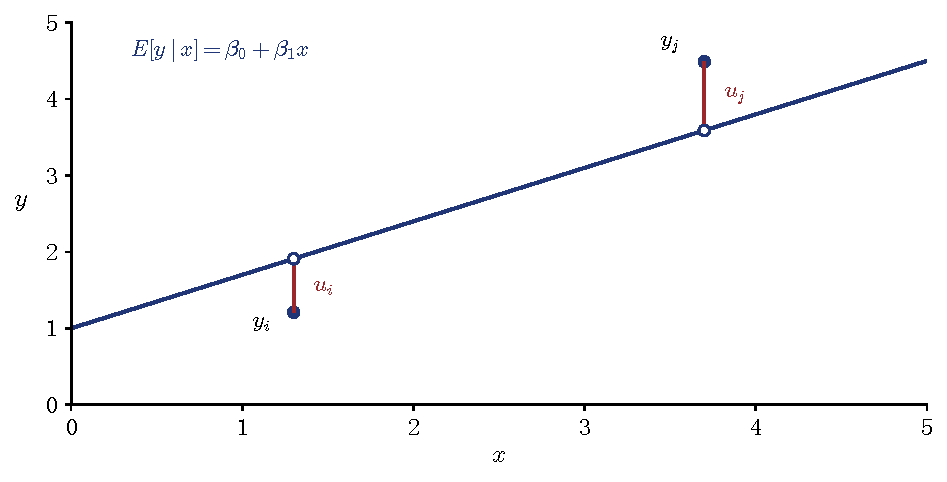
\includegraphics[width=.79\linewidth]{population_errors.pdf}
\caption{Population errors are vertical deviations from the conditional mean, not residuals from an estimated line. This redraw follows the two-observation sketch; the observations are schematic.}
\label{fig:population-errors}
\end{figure}

\paragraph{SLR3: variation in the regressor.}
The observed $x_i$ cannot all take the same value:
\[\hy{$S_{xx}=\sum_i(x_i-\bar x)^2>0$}.\]
If all $x_i$ coincide, the slope formula has a zero denominator and the separate intercept and slope cannot be recovered.

\paragraph{SLR4: zero conditional mean.}
\[\hy{$\E[u_i\mid x_i]=0$}\qquad(i=1,\ldots,n).\]
The average unobserved component is zero at each value of the explanatory variable. Under independent sampling this also implies
\[\E[u_i\mid\mathcal X]=0,\qquad\mathcal X=(x_1,\ldots,x_n),\]
because the other observations' regressors provide no additional information about $u_i$ once $x_i$ is known. Conditioning on the \emph{whole observed design} is needed in the proof, because $S_{xx}$ is random before sampling.\corr{conditioning}

\begin{theorem}[Unbiasedness of simple OLS]\label{thm:simple-unbiased}
Under SLR1--SLR4 and the existence conditions above,
\[\E[\hat\beta_0\mid\mathcal X]=\beta_0,\qquad
\E[\hat\beta_1\mid\mathcal X]=\beta_1.\]
Consequently $\E[\hat\beta_0]=\beta_0$ and $\E[\hat\beta_1]=\beta_1$.
\end{theorem}

\subsection{Proof for the slope}
Expand the slope formula step by step:
\begin{align}
\hat\beta_1
&=\frac{\sum_i(x_i-\bar x)(y_i-\bar y)}{S_{xx}}
=\frac{\sum_i(x_i-\bar x)y_i}{S_{xx}}\notag\\
&=\frac{\sum_i(x_i-\bar x)(\beta_0+\beta_1x_i+u_i)}{S_{xx}}\notag\\
&=\frac{\beta_0\sum_i(x_i-\bar x)
+\beta_1\sum_i(x_i-\bar x)x_i+\sum_i(x_i-\bar x)u_i}{S_{xx}}.\label{eq:slope-expansion}
\end{align}
Now $\sum_i(x_i-\bar x)=0$, and
\begin{align*}
S_{xx}&=\sum_i(x_i^2-2x_i\bar x+\bar x^2)
=\sum_i x_i^2-n\bar x^2\\
&=\sum_i x_i(x_i-\bar x).
\end{align*}
Hence
\begin{equation}\label{eq:slope-error}
\hm{\hat\beta_1=\beta_1+\frac{\sum_i(x_i-\bar x)u_i}{S_{xx}}}.
\end{equation}
\begin{align*}
\E[\hat\beta_1\mid\mathcal X]
&=\beta_1+\frac{\sum_i(x_i-\bar x)\E[u_i\mid\mathcal X]}{S_{xx}}\\
&=\beta_1.
\end{align*}
Finally, $\E[\hat\beta_1]=\E\{\E[\hat\beta_1\mid\mathcal X]\}=\beta_1$. \red{不能在无条件期望中直接把随机分母 $S_{xx}$ 提到期望外。}\corr{conditioning}

\subsection{Proof for the intercept: Exam}
\sourcepage{4}{3}{4/3}
\label{sec:intercept-proof}
By the model and sample averaging,
\[\bar y=\beta_0+\beta_1\bar x+\bar u,\qquad
\bar u=\frac1n\sum_i u_i.\]
Substitute this into $\hat\beta_0=\bar y-\hat\beta_1\bar x$:
\[\hat\beta_0=\beta_0+(\beta_1-\hat\beta_1)\bar x+\bar u.\]
Thus
\begin{align*}
\E[\hat\beta_0\mid\mathcal X]
&=\beta_0+\bar x\bigl(\beta_1-\E[\hat\beta_1\mid\mathcal X]\bigr)
+\E[\bar u\mid\mathcal X]\\
&=\beta_0+\bar x(\beta_1-\beta_1)+0=\beta_0.
\end{align*}
The $\bar u$ term enters with a \emph{plus} sign; the handwritten proof contains an inconsistent intermediate minus sign, corrected here.\corr{intercept-sign}
Iterated expectations then gives $\E[\hat\beta_0]=\beta_0$.

\subsection{Discussion: what if assumptions are violated?}
\blue{原稿在此处另有课堂时间标记：15 分钟。}
\begin{description}
\item[SLR1: linear in parameters.] A model nonlinear in the unknown coefficients falls outside this particular linear-OLS proof. \blue{非线性参数与变量的非线性变换要区分。}
\item[SLR2: random sampling.] The source lists serial correlation (autocorrelation) in time series, unrepresentative samples, and spillover effects across observations. These invalidate the stated i.i.d. setup, or raise representativeness and model concerns. They do \emph{not} by themselves prove that every OLS coefficient is biased; conditional mean restrictions must be examined separately.\corr{violations}
\item[SLR3: sample variation.] If $S_{xx}=0$, the simple slope is not identified separately from the intercept.
\item[SLR4: zero conditional mean.] In observational settings omitted factors may be related to regressors. If $\Cov(x,u)\ne0$, ZCM cannot hold. But ZCM is stronger than zero covariance: $\Cov(x,u)=0$ does not imply $\E[u\mid x]=0$. A failure of ZCM alone does not logically guarantee a nonzero finite-sample bias in every possible design.\corr{zcm-covariance}
\end{description}
\added{The source's covariance identity is
\[\Cov(x,u)=\E[xu]-\E[x]\E[u].\]
ZCM implies both $\E[u]=0$ and $\E[xu]=0$, subject to moment existence. The reverse implication is not generally valid.}

\section{Multiple OLS: Assumptions and Theorem}
\sourcepage{4}{4}{4/5}
\label{sec:multiple-unbiased}
\subsection{MLR1: linear in parameters}
The population model is
\[y=\beta_0+\beta_1x_1+\beta_2x_2+\cdots+\beta_kx_k+u.\]
The coefficients $\beta_0,\ldots,\beta_k$ are unknown constants of interest; $u$ is the error term.

\subsection{MLR2: random sampling}
There is an i.i.d. sample of $n$ observation vectors
\[\{(x_{1i},\ldots,x_{ki},y_i):i=1,\ldots,n\}\]
from this population model, so $y_i=\beta_0+\sum_{j=1}^k\beta_jx_{ji}+u_i$.

\subsection{MLR3: no perfect collinearity}
The sample design, including its intercept column, has full column rank. No non-intercept regressor is constant, and no regressor is an exact linear combination of the other columns. \blue{相关可以存在；完全线性的重复信息会使单独系数无法识别。}

\begin{example}[Perfect collinearity]
The original examples are retained:
\begin{enumerate}
\item A constant regressor: $x_1=10$ in a model already containing an intercept.
\item Exact scaling or an affine relation: $x_1=2x_2$, or $x_1=a+bx_2$.
\item An exact linear combination: $x_3=x_1+x_2$.
\end{enumerate}
\begin{figure}[htbp]
\centering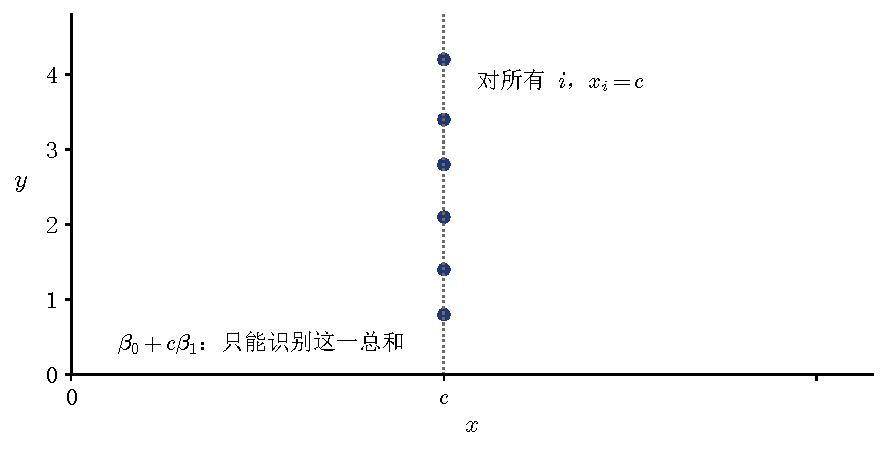
\includegraphics[width=.72\linewidth]{no_sample_variation.pdf}
\caption{If $x_i=c$ for every observation, only $\beta_0+c\beta_1$ is identified. This reproduces the source's constant-$x$ sketch using schematic points.}
\label{fig:no-variation}
\end{figure}
In a regression containing $\ln(\mathrm{income})$, adding $2\ln(\mathrm{income})$ creates perfect collinearity. Likewise, a model containing expenditure A, expenditure B and total expenditure is collinear when total expenditure $=$ expenditure A $+$ expenditure B.

Keeping expenditure A and B but omitting their exact total does not itself create this particular collinearity. The specification
\[y=\beta_0+\beta_1\ln(\mathrm{income})
+\beta_2[\ln(\mathrm{income})]^2+u\]
is not \emph{automatically} perfectly collinear: a squared regressor is generally not an affine transformation of its level. \blue{它对变量可以非线性，但对参数仍线性。} Special samples with too few distinct values can still fail full rank.\corr{collinearity}
\end{example}


\subsection{MLR4: zero conditional mean}
\sourcepage{4}{5}{4/6}
\[\hm{\E[u\mid x_1,x_2,\ldots,x_k]=0}.\]
The explanatory variables do not systematically predict the error's conditional mean. In the terminology used in these notes, this is the mean-exogeneity condition. \red{它推出与误差不相关；仅仅不相关不足以推出这个条件。}\corr{zcm-covariance}
The source contrasts exogenous and endogenous regressors. In a structural model, regressors related to omitted determinants in $u$ can be endogenous; a zero sample covariance with \emph{fitted residuals} is not evidence against that problem.

\begin{theorem}[Unbiasedness of multiple OLS]\label{thm:multiple-unbiased}
Under MLR1--MLR4, almost-sure full rank and the existence of the relevant expectations,
\[\E[\hat\beta_j\mid\mathcal X]=\beta_j,
\qquad\E[\hat\beta_j]=\beta_j,\qquad j=0,1,\ldots,k,\]
where $\mathcal X$ denotes the entire observed regressor matrix.
\end{theorem}

\subsection{Proof using partialling out / 控制其他因素}
\label{sec:fwl-week4}
Fix a regressor $x_j$. Following the source, regress it on a constant and all the other regressors:
\begin{equation}\label{eq:auxiliary-j}
x_{ji}=\hat\delta_0+\sum_{\ell\ne j}\hat\delta_\ell x_{\ell i}+\hat r_{ji}.
\end{equation}
\blue{不同样本会有不同的辅助回归系数和残差。给定整组 $\mathcal X$，这些量都是已确定的。}
The auxiliary normal equations give
\[\sum_i\hat r_{ji}=0,\qquad
\sum_i x_{\ell i}\hat r_{ji}=0\quad(\ell\ne j).\]
Define the \emph{auxiliary} residual sum of squares
\[S_{r_jr_j}=\sum_i\hat r_{ji}^{\,2}>0.
\]
It is the source's ``$\RSS_j$'', distinct from the residual sum of squares of the outcome regression. Since $x_{ji}$ equals its fitted auxiliary component plus $\hat r_{ji}$,
\[\sum_i\hat r_{ji}x_{ji}=\sum_i\hat r_{ji}^{\,2}=S_{r_jr_j}.
\]
FWL, in its one-sided coefficient form, gives
\begin{align}
\hat\beta_j
&=\frac{\Cov_n(\hat r_j,y)}{\Var_n(\hat r_j)}
=\frac{\sum_i\hat r_{ji}y_i}{S_{r_jr_j}}\notag\\
&=\frac{\sum_i\hat r_{ji}\left(\beta_0+\sum_{\ell=1}^k\beta_\ell x_{\ell i}+u_i\right)}{S_{r_jr_j}}\notag\\
&=\hm{\beta_j+\frac{\sum_i\hat r_{ji}u_i}{S_{r_jr_j}}}.\label{eq:multiple-slope-error}
\end{align}
All the other-regressor terms vanish by auxiliary orthogonality. Taking conditional expectations,
\[\E[\hat\beta_j\mid\mathcal X]
=\beta_j+\frac{\sum_i\hat r_{ji}\E[u_i\mid\mathcal X]}{S_{r_jr_j}}
=\beta_j.\]
Iterated expectations proves the unconditional result for every slope.
\added{The intercept follows from
\[\hat\beta_0=\bar y-\sum_{j=1}^k\hat\beta_j\bar x_j
=\beta_0+\bar u+\sum_{j=1}^k(\beta_j-\hat\beta_j)\bar x_j.\]
Conditioning on $\mathcal X$ makes every $\bar x_j$ fixed; the slope result and $\E[\bar u\mid\mathcal X]=0$ then give $\E[\hat\beta_0\mid\mathcal X]=\beta_0$.}

\section{Assumptions Summary and Unbiasedness}
\sourcepage{4}{6}{4/7}
\label{sec:assumptions-summary}
\paragraph{核心：controlling for.}
多元回归的核心能力是通过 FWL 排除其他已观测因素的线性影响，识别某一自变量剩余变化与结果的关系。\blue{“纯净影响”的因果说法仍依赖适当的模型与外生性，不能仅由控制操作保证。}

\paragraph{无偏性的本质：重复抽样的平均性质.}
单次抽样的具体估计是一个已经实现的数值；生成这些数值的 OLS 估计程序才有统计意义上的无偏性。

\subsection{The four assumptions side by side}
\begin{center}
\small\renewcommand{\arraystretch}{1.35}
\begin{tabular}{P{3.1cm}P{5.35cm}P{6.3cm}}
\toprule
Assumption & Simple regression & Multiple regression\\
\midrule
Linearity in parameters & $y=\beta_0+\beta_1x+u$ & $y=\beta_0+\sum_{j=1}^k\beta_jx_j+u$\\
Random sampling & i.i.d. pairs $(x_i,y_i)$ & i.i.d. vectors $(x_{1i},\ldots,x_{ki},y_i)$\\
Sample rank & $\sum_i(x_i-\bar x)^2>0$ & No exact linear relationship among the design columns, including the constant\\
Zero conditional mean & $\E[u\mid x]=0$ & $\E[u\mid x_1,\ldots,x_k]=0$\\
\bottomrule
\end{tabular}
\end{center}

\begin{example}[A realised education-return estimate]\label{ex:unbiased-number}
The source gives
\[\widehat{\ln(\wage)}
=0.284+0.092\educ+0.0041\,\mathrm{exper}+0.022\,\mathrm{tenure}.\]
If MLR1--MLR4 hold, can we say ``9.2\% is an unbiased estimate of the return to education''?

\red{The relevant property belongs to the estimator.} The number $0.092$ is one realised estimate. A precise statement is that the OLS estimator of the log-wage coefficient is unbiased under the stated assumptions; its realisation in this sample is $0.092$.

The source's ``9.2\%'' is the approximate one-year percentage interpretation. The exact constant-error percentage transformation is
\[100(e^{0.092}-1)\simeq9.64\%.
\]
\added{Even if $\hat\beta$ is unbiased for $\beta$, the nonlinear transform $e^{\hat\beta}-1$ need not be unbiased for $e^\beta-1$. Also, fitting log wages does not by itself identify a causal education return or the conditional mean of wages in levels.}\corr{unbiased-log}
\end{example}

\section{Model Specification and Bias}
\sourcepage{4}{7}{4/8}
\label{sec:model-specification}
There are two specification cases: \hy{overspecification}, including irrelevant variables; and \hy{underspecification}, omitting relevant variables.

\subsection{Including an irrelevant variable}
Start from
\[y=\beta_0+\beta_1x_1+\beta_2x_2+u.\]
Now estimate a model also containing $x_3$, with its population coefficient $\beta_3=0$. The expanded sample must retain full rank: $x_3$ must not be an exact linear combination of the existing design columns.

If the \emph{expanded} exogeneity condition holds,
\[\E[u\mid x_1,x_2,x_3]=0,
\]
then the full-model OLS estimators remain unbiased:
\[\E[\hat\beta_j]=\beta_j\quad(j=0,1,2),\qquad
\E[\hat\beta_3]=0.
\]
\red{But $\E[u\mid x_1,x_2]=0$ alone does not imply $\E[u\mid x_1,x_2,x_3]=0$.} Adding a regressor associated with the error can change the conditional-mean restriction. An irrelevant coefficient is not, on its own, proof that this additional control is exogenous.\corr{irrelevant-exogeneity}

\added{Under the homoskedastic fixed-design model, including an irrelevant regressor weakly increases the conditional variance of an existing slope when it reduces that regressor's residual variation. It need not strictly increase it, and a realised estimated standard error need not rise. The original note's ``variance increases'' is read with these qualifications.}\corr{irrelevant-variance}

\subsection{Omitting a relevant variable}
\label{sec:ovb-sample}
Let the true long model be
\[y_i=\beta_0+\beta_1x_i+\beta_2z_i+u_i,\qquad
\E[u_i\mid x_i,z_i]=0.\]
Its fitted version is
\[y_i=\hat\beta_0+\hat\beta_1x_i+\hat\beta_2z_i+\hat u_i.
\]
If $z$ is unobserved or omitted, the short regression fits $y$ on $(1,x)$:
\[y_i=\hat{\tilde\beta}_0+\hat{\tilde\beta}_1x_i+\hat v_i,
\qquad v_i=\beta_2z_i+u_i\ \text{in the structural equation}.
\]
Omitting a relevant variable is problematic for the slope on $x$ when the omitted component is related to $x$; relevance alone is not enough.\corr{omitting-relevant}

\paragraph{Exact sample short--long identity.}
The exact sample relation is
\begin{equation}\label{eq:sample-ovb}
\hm{\hat{\tilde\beta}_1=\hat\beta_1+\hat\beta_2\hat\delta_1},
\end{equation}
where $\hat\delta_1$ comes from the auxiliary OLS regression
\[z_i=\hat\delta_0+\hat\delta_1x_i+\hat r_i,
\qquad
\hat\delta_1=\frac{\sum_i(x_i-\bar x)(z_i-\bar z)}{S_{xx}}.
\]
First, the long-model residual is sample-orthogonal to $x$ and the constant:
\begin{align*}
\sum_i(x_i-\bar x)(\hat u_i-\bar{\hat u})
&=\sum_i x_i\hat u_i-\bar x\sum_i\hat u_i\\
&=0.
\end{align*}
Substituting the demeaned long fitted equation into the short slope formula gives
\begin{align*}
\hat{\tilde\beta}_1
&=\frac{\sum_i(x_i-\bar x)(y_i-\bar y)}{S_{xx}}\\
&=\frac{\sum_i(x_i-\bar x)\left[\hat\beta_1(x_i-\bar x)
+\hat\beta_2(z_i-\bar z)+(\hat u_i-\bar{\hat u})\right]}{S_{xx}}\\
&=\hat\beta_1+\hat\beta_2\frac{\sum_i(x_i-\bar x)(z_i-\bar z)}{S_{xx}}+0\\
&=\hat\beta_1+\hat\beta_2\hat\delta_1.
\end{align*}
This is an algebraic identity for the same realised sample; it does not yet take expectations.

\subsection{Expected bias: which quantities are random?}
\sourcepage{4}{8}{4/9}
\label{sec:ovb-expectation}
Let $\mathcal X$ now include all sampled $x_i$ and $z_i$. Under the valid long model,
\[\E[\hat\beta_1\mid\mathcal X]=\beta_1,
\qquad\E[\hat\beta_2\mid\mathcal X]=\beta_2.
\]
The auxiliary slope $\hat\delta_1$ is fixed \emph{given} this design. Thus
\begin{align}
\E[\hat{\tilde\beta}_1\mid\mathcal X]
&=\E[\hat\beta_1+\hat\beta_2\hat\delta_1\mid\mathcal X]\notag\\
&=\hm{\beta_1+\beta_2\hat\delta_1},\label{eq:ovb-conditional}\\
\E[\hat{\tilde\beta}_1]
&=\beta_1+\beta_2\E[\hat\delta_1].\label{eq:ovb-unconditional}
\end{align}
Equivalently, retaining the source's iterated-expectation route,
\begin{align*}
\E[\hat\beta_2\hat\delta_1]
&=\E\{\E[\hat\beta_2\hat\delta_1\mid\mathcal X]\}\\
&=\E\{\hat\delta_1\E[\hat\beta_2\mid\mathcal X]\}
=\beta_2\E[\hat\delta_1].
\end{align*}
\added{To obtain the source's finite-sample expression
\[\E[\hat{\tilde\beta}_1]=\beta_1+\beta_2\delta_1,\]
one also needs $\E[\hat\delta_1]=\delta_1$. A sufficient additional condition is a correctly specified auxiliary conditional mean
\[\E[z\mid x]=\delta_0+\delta_1x\]
with random sampling, sample variation and the requisite integrability. Defining $\delta_1$ only as the population projection slope does not automatically establish this finite-sample equality.}\corr{ovb-levels}

For the \emph{population linear projection}, without imposing this additional linear conditional mean, the slope difference is still
\[\tilde\beta_1-\beta_1=\beta_2\delta_1,
\qquad\delta_1=\frac{\Cov(x,z)}{\Var(x)}.
\]
Under the usual consistency conditions it also describes the asymptotic slope difference. These population and asymptotic statements should not be confused with the exact sample identity or a finite-sample expectation.

\subsection{Direction of omitted-variable bias}
When the applicable slope difference or bias is $B=\beta_2\delta_1$,
\begin{description}
\item[Upward.] $B>0$: the short slope is higher than the target $\beta_1$.
\item[Downward.] $B<0$: the short slope is lower than the target $\beta_1$.
\item[Zero.] $B=0$, for example $\beta_2=0$ or $\delta_1=0$.
\end{description}
For $\Var(x)>0$, the sign of $\delta_1$ is the sign of $\Cov(x,z)$. The original sign table becomes
\begin{center}
\renewcommand{\arraystretch}{1.4}
\begin{tabular}{lcc}
\toprule
 & $\Cov(x,z)>0$ ($\delta_1>0$) & $\Cov(x,z)<0$ ($\delta_1<0$)\\
\midrule
$\beta_2>0$ & \hy{Upward} & Downward\\
$\beta_2<0$ & Downward & \hy{Upward}\\
\bottomrule
\end{tabular}
\end{center}
\blue{该表直接适用于总体投影差；用于有限样本平均偏差时，应满足上一小节的附加条件。给定样本设计的偏差方向则由 $\hat\delta_1$ 决定。}

\paragraph{Biased toward zero / 向零偏.}
For a positive $\beta_1$, movement toward zero is downward; for a negative $\beta_1$, it is upward. To use the usual attenuation interpretation, the shifted coefficient must remain between the target and zero. \red{方向正确但越过零，不能仅凭 upward/downward 就称为向零偏。}\corr{toward-zero}

\subsection*{Chapter recap / 本章小结}
\addcontentsline{toc}{subsection}{Chapter recap / 本章小结}
\begin{itemize}
\item Unbiasedness is an expectation property of the estimator over repeated samples.
\item Full-rank sample variation and zero conditional mean underpin the conditional-expectation proof; mere zero covariance is weaker.
\item Adding a valid irrelevant control preserves unbiasedness but can cost precision. Omitting a relevant, associated regressor changes the slope.
\item Keep sample identities, conditional bias, unconditional finite-sample bias and population projection differences distinct.
\end{itemize}

\appendix
\chapter{原稿对应表}
\label{app:sources}
每行对应一页原始 PDF；点击正文页码可跳到该页内容开始的位置。跨页内容仍按原稿顺序衔接。所有 23 页均逐页查看，原稿中的重复讲解、例式和页底可见片段均保留。
第 4 周的手写页码跳号按用户说明属于练习安排，不标记为漏扫；不补写未提供的练习。第 2 周末页的手写页码以 PDF 第 8 页定位，避免猜写最后一位。
\small\renewcommand{\arraystretch}{1.25}
\begin{longtable}{P{1.05cm}P{.8cm}P{2.25cm}P{9.7cm}P{.9cm}}
\toprule 周次 & PDF & 手写页码 & 已整理内容 & 页码\\\midrule\endfirsthead
\toprule 周次 & PDF & 手写页码 & 已整理内容 & 页码\\\midrule\endhead
\bottomrule\endfoot
2 & 1 & 2/1 & 简单模型；其他条件不变；误差归一化；零条件均值；工资例题 & \hyperref[src:w2p1]{\pageref*{src:w2p1}}\\
2 & 2 & 2/2 & 总体回归函数推导；OLS 系数；相关与因果；截距；薪酬示意图 & \hyperref[src:w2p2]{\pageref*{src:w2p2}}\\
2 & 3 & 2/3 & 工资单位练习；安森的假设情景；得票与竞选支出练习 & \hyperref[src:w2p3]{\pageref*{src:w2p3}}\\
2 & 4 & 2/4 & 多元偏效应；相关的控制变量；平均绩点解释；安森与贝蒂 & \hyperref[src:w2p4]{\pageref*{src:w2p4}}\\
2 & 5 & 2/5 & 控制变量；能力；保持不变；单侧及一般 FWL 定理 & \hyperref[src:w2p5]{\pageref*{src:w2p5}}\\
2 & 6 & 2/6 & 短回归与长回归；系数相同的条件；舍入后的绩点方程 & \hyperref[src:w2p6]{\pageref*{src:w2p6}}\\
2 & 7 & 2/7 & 因变量与自变量单位变换；截距解释；样本协方差推导 & \hyperref[src:w2p7]{\pageref*{src:w2p7}}\\
2 & 8 & 末页，按 PDF 定位 & 水平值与对数的四类模型；百分比解释 & \hyperref[src:w2p8]{\pageref*{src:w2p8}}\\
3 & 1 & 3/1 & 误差与残差；简单 OLS 的三个样本性质；总体矩条件 & \hyperref[src:w3p1]{\pageref*{src:w3p1}}\\
3 & 2 & 3/2 & 三类平方和；交叉项证明；完全拟合；判定系数的相关解释 & \hyperref[src:w3p2]{\pageref*{src:w3p2}}\\
3 & 3 & 3/3 & 判定系数比较图；再次保留多元 OLS 性质及证明 & \hyperref[src:w3p3]{\pageref*{src:w3p3}}\\
3 & 4 & 3/4 & 增加回归变量；调整判定系数；绩点数值核算；三点提醒 & \hyperref[src:w3p4]{\pageref*{src:w3p4}}\\
3 & 5 & 3/5 & 过原点估计；去均值；均值点示意图；页底重复的工资例式 & \hyperref[src:w3p5]{\pageref*{src:w3p5}}\\
3 & 6 & 补充推导页 & 再次保留有无截距的公式；去均值；仅含常数项的回归；FWL & \hyperref[src:w3p6]{\pageref*{src:w3p6}}\\
3 & 7 & 3/6 & 再次保留过原点回归一阶条件；样本性质；协方差限制；负判定系数 & \hyperref[src:w3p7]{\pageref*{src:w3p7}}\\
4 & 1 & 4/1 & 学习目标；估计回顾；参数与估计量；无偏性；简单回归假设概览 & \hyperref[src:w4p1]{\pageref*{src:w4p1}}\\
4 & 2 & 4/2 & 简单回归假设详解；总体误差示意图；斜率无偏性的证明 & \hyperref[src:w4p2]{\pageref*{src:w4p2}}\\
4 & 3 & 4/3 & 考试提示中的截距证明；违背假设的后果及结论边界 & \hyperref[src:w4p3]{\pageref*{src:w4p3}}\\
4 & 4 & 4/5 & 多元回归前三项假设；常数自变量示意图；全部完全共线性例子 & \hyperref[src:w4p4]{\pageref*{src:w4p4}}\\
4 & 5 & 4/6 & 多元回归第四项假设；无偏性定理；辅助残差性质；FWL 期望证明 & \hyperref[src:w4p5]{\pageref*{src:w4p5}}\\
4 & 6 & 4/7 & 控制变量与无偏性回顾；假设对照表；某次对数工资估计 & \hyperref[src:w4p6]{\pageref*{src:w4p6}}\\
4 & 7 & 4/8 & 无关控制变量；遗漏相关变量；短长回归的精确样本恒等式 & \hyperref[src:w4p7]{\pageref*{src:w4p7}}\\
4 & 8 & 4/9 & 迭代期望偏误证明；附加条件；偏误方向与符号表 & \hyperref[src:w4p8]{\pageref*{src:w4p8}}\\
\end{longtable}\normalsize
\section*{复现与原件}
原始 PDF 和 BMO 模板副本保持原样；文件路径、字节数及 SHA256 校验值见项目中的 sources/manifest.json。矢量图和对应预览由同一 Python 脚本生成，数值检查记录另保存在 qa 目录。

\chapter{勘误与补充说明}

\label{app:errata}

正文直接采用正确写法；本附录记录实质修正及必要条件补充。原稿本来正确的结论不因列入此处而被视为错误；部分条目只是限制适用范围或明确记号。点原稿定位可返回正文；未删除原稿学习内容。

\section*{核对依据}

\begin{description}

\item[H1.] 汉森，\emph{计量经济学}，2010 年 1 月 10 日稿，第 2 章：条件均值、投影与解释。 \href{https://users.ssc.wisc.edu/~xshi28/Econometrics_Hansen.pdf}{大学网站公开的教材手稿}.

\item[H2.] 同一手稿，第 3.3 至 3.7 节及第 3.10 节：OLS 代数、残差回归与拟合优度。

\item[H3.] 同一手稿，第 4.3、4.4、4.11、4.12 节：条件无偏性、方差、共线性与遗漏变量。本笔记还明确推导了额外的有限样本限定条件。

\item[M.] 梅西大学， \href{https://r-resources.massey.ac.nz/161251/lectures/RegressionOrigin.html}{\emph{过原点回归}}: 中心化与非中心化拟合统计量的比较。

\item[计算.] 对原稿算式直接进行代数推导或数值运算；项目中包含可复现的数值核对。

\end{description}

外部材料仅用于核对数学与适用条件；本次排版模板仍是用户指定的旧 BMO 笔记。

\par\medskip\noindent\begin{minipage}{\linewidth}

\phantomsection\label{err:notation}

\textbf{C01. 总体、估计量与拟合值记号}\quad\textbf{原稿定位：}\hyperref[src:w2p4]{第 2 周，PDF 第 4 页}；\hyperref[src:w3p1]{第 3 周，PDF 第 1 页}。\quad\textbf{核对：}H1。\par

总体参数写作 $\beta_j$，样本估计写作 $\hat\beta_j$；总体误差 $u_i$ 与残差 $\hat u_i$ 分开。拟合值变化使用 $\Delta\hat y$，不将 $\hat\beta_j$ 直接写成总体参数。

\end{minipage}\par

\par\medskip\noindent\begin{minipage}{\linewidth}

\phantomsection\label{err:mean-normalisation}

\textbf{C02. 误差均值的归一化}\quad\textbf{原稿定位：}\hyperref[src:w2p1]{第 2 周，PDF 第 1 页}。\quad\textbf{核对：}H1。\par

令 $\varepsilon=u-\alpha$ 后，$\E[\varepsilon]=0$，而不是 $\varepsilon$ 处处等于零。截距变为 $\beta_0+\alpha$。该归一化本身不保证零条件均值。

\end{minipage}\par

\par\medskip\noindent\begin{minipage}{\linewidth}

\phantomsection\label{err:slope-correlation}

\textbf{C03. 斜率与相关系数的比例}\quad\textbf{原稿定位：}\hyperref[src:w2p2]{第 2 周，PDF 第 2 页}。\quad\textbf{核对：}H2。\par

样本简单 OLS 斜率为 $r_{xy}s_y/s_x$，不是 $r_{xy}s_x/s_y$；总体投影系数和样本系数不能混用。

\end{minipage}\par

\par\medskip\noindent\begin{minipage}{\linewidth}

\phantomsection\label{err:causality}

\textbf{C04. 相关与因果的边界}\quad\textbf{原稿定位：}\hyperref[src:w2p2]{第 2 周，PDF 第 2 页}；\hyperref[src:w2p4]{第 2 周，PDF 第 4 页}。\quad\textbf{核对：}H1。\par

保留“相关联”的措辞；控制变量、ZCM 或好的拟合度本身不能替代结构模型与可辩护的因果识别。截距在 $x=0$ 不可行时只是外推。

\end{minipage}\par

\par\medskip\noindent\begin{minipage}{\linewidth}

\phantomsection\label{err:wage-counterfactual}

\textbf{C05. 工资题中的单位与个体反事实}\quad\textbf{原稿定位：}\hyperref[src:w2p3]{第 2 周，PDF 第 3 页}。\quad\textbf{核对：}计算。\par

按原稿“千美元”复算：$5.58$、$-5.574$、$7.74$、$2.166$ 均使用同一单位。固定该人残差得到的是模型情景，并非保证的实际工资。未把看似异常的原题单位擅自改成美元。

\end{minipage}\par

\par\medskip\noindent\begin{minipage}{\linewidth}

\phantomsection\label{err:election}

\textbf{C06. 选举题的比例与金额}\quad\textbf{原稿定位：}\hyperref[src:w2p3]{第 2 周，PDF 第 3 页}。\quad\textbf{核对：}计算。\par

40\% 应输入 40，预测为 45.37\%；50\% 的预测阈值对应 支出占比 $>49.978448\ldots$。补齐在 B 支出 20 亿美元时 A 的支出阈值，区别预测过半与实际获胜。

\end{minipage}\par

\par\medskip\noindent\begin{minipage}{\linewidth}

\phantomsection\label{err:fwl-residual}

\textbf{C07. FWL 的单侧与双侧残差化}\quad\textbf{原稿定位：}\hyperref[src:w2p5]{第 2 周，PDF 第 5 页}；\hyperref[src:w4p5]{第 4 周，PDF 第 5 页}。\quad\textbf{核对：}H2。\par

只残差化自变量后回归原始 $y$，系数相同，但残差一般不等于原多元模型残差。对 $y$ 与该自变量同时排除其他回归量，才能同时得到相同系数与残差。

\end{minipage}\par

\par\medskip\noindent\begin{minipage}{\linewidth}

\phantomsection\label{err:ovb-levels}

\textbf{C08. 遗漏变量公式的三个层次}\quad\textbf{原稿定位：}\hyperref[src:w2p6]{第 2 周，PDF 第 6 页}；\hyperref[src:w4p8]{第 4 周，PDF 第 8 页}。\quad\textbf{核对：}H3。\par

保留样本恒等式 $\hat{\tilde\beta}_1=\hat\beta_1+\hat\beta_2\hat\delta_1$。给定整组设计时，偏差为 $\beta_2\hat\delta_1$；无条件有限样本偏差为 $\beta_2\E[\hat\delta_1]$。写成 $\beta_2\delta_1$ 还须有辅助斜率无偏等附加条件；总体投影差另行说明。

\end{minipage}\par

\par\medskip\noindent\begin{minipage}{\linewidth}

\phantomsection\label{err:unit-intercept}

\textbf{C09. 换单位时的截距与条件均值}\quad\textbf{原稿定位：}\hyperref[src:w2p7]{第 2 周，PDF 第 7 页}。\quad\textbf{核对：}计算。\par

总体截距的含义是 $\E[y\mid x=0]$，不是一般的 $\E[y]$；$y$ 乘以 $c$ 时截距也乘以 $c$。$x$ 乘以非零 $c$ 时斜率除以 $c$，截距不变。

\end{minipage}\par

\par\medskip\noindent\begin{minipage}{\linewidth}

\phantomsection\label{err:logs}

\textbf{C10. 有限变化与对数近似}\quad\textbf{原稿定位：}\hyperref[src:w2p8]{第 2 周，PDF 第 8 页}。\quad\textbf{核对：}计算。\par

将有限变化的近似与精确关系分开。水平值—对数模型为 $\beta_1\ln(x_1/x_0)$；对数—水平值模型的精确百分比为 $100(e^{\beta_1\Delta x}-1)$；对数—对数模型使用比例的幂。对数模型的系数仍保留原稿的局部百分比解释。

\end{minipage}\par

\par\medskip\noindent\begin{minipage}{\linewidth}

\phantomsection\label{err:sample-population}

\textbf{C11. 样本恒等式不是总体外生性的检验}\quad\textbf{原稿定位：}\hyperref[src:w3p1]{第 3 周，PDF 第 1 页}。\quad\textbf{核对：}H2。\par

残差和为零、与包含的回归量正交来自样本 OLS 一阶条件。不能从这些条件推出真实误差的 ZCM。总体均值关系用无帽参数，样本均值关系用样本系数。

\end{minipage}\par

\par\medskip\noindent\begin{minipage}{\linewidth}

\phantomsection\label{err:r2-degenerate}

\textbf{C12. 判定系数 的退化情形}\quad\textbf{原稿定位：}\hyperref[src:w3p2]{第 3 周，PDF 第 2 页}。\quad\textbf{核对：}H2。\par

补充 TSS 必须大于零。拟合值恒定时，普通 $R^2$ 可以为零，但相关系数因分母为零而未定义；此时不能直接用相关系数平方计算。

\end{minipage}\par

\par\medskip\noindent\begin{minipage}{\linewidth}

\phantomsection\label{err:r2-rss}

\textbf{C13. 高拟合度与 RSS 的比较}\quad\textbf{原稿定位：}\hyperref[src:w3p3]{第 3 周，PDF 第 3 页}。\quad\textbf{核对：}H2。\par

高 $R^2$ 表示较小的 RSS/TSS；不能跨不同样本或单位仅凭较高 $R^2$ 就认定绝对 RSS 更小。图中 0.94 和 0.64 均由新绘制的示意点实际计算。

\end{minipage}\par

\par\medskip\noindent\begin{minipage}{\linewidth}

\phantomsection\label{err:r2-monotonic}

\textbf{C14. 增加回归量时 判定系数 不减}\quad\textbf{原稿定位：}\hyperref[src:w3p4]{第 3 周，PDF 第 4 页}。\quad\textbf{核对：}H2。\par

原稿的“增加”改为“不下降，可以保持不变”，并注明必须是相同观测、相同因变量的嵌套 OLS 比较。不同缺失值样本不在该结论内。

\end{minipage}\par

\par\medskip\noindent\begin{minipage}{\linewidth}

\phantomsection\label{err:adjusted-meaning}

\textbf{C15. 调整判定系数 的提高条件}\quad\textbf{原稿定位：}\hyperref[src:w3p4]{第 3 周，PDF 第 4 页}。\quad\textbf{核对：}计算。\par

“变量有意义才提高”改写为残差均方必须下降；增加 $q$ 个回归量时，对应描述性的 偏 F 统计量 大于 1。这个阈值不是常规显著性检验，也不证明因果。

\end{minipage}\par

\par\medskip\noindent\begin{minipage}{\linewidth}

\phantomsection\label{err:demeaning}

\textbf{C16. 去均值与过原点回归}\quad\textbf{原稿定位：}\hyperref[src:w3p5]{第 3 周，PDF 第 5 页}；\hyperref[src:w3p6]{第 3 周，PDF 第 6 页}。\quad\textbf{核对：}H2。\par

是“去均值后无截距”的斜率等于“原始数据带截距”的斜率；不是任意无截距回归都等于带截距回归。原稿的两次推导均保留。

\end{minipage}\par

\par\medskip\noindent\begin{minipage}{\linewidth}

\phantomsection\label{err:rto-covariance}

\textbf{C17. 无截距时的正交与不相关}\quad\textbf{原稿定位：}\hyperref[src:w3p7]{第 3 周，PDF 第 7 页}。\quad\textbf{核对：}H2。\par

$\sum_i x_i\check u_i=0$ 仍成立，但 $\Cov_n(x,\check u)=-\bar x\bar{\check u}$ 一般不为零。原稿将两者等同的说法已改正。

\end{minipage}\par

\par\medskip\noindent\begin{minipage}{\linewidth}

\phantomsection\label{err:rto-cross-term}

\textbf{C18. 平方和分解的交叉项}\quad\textbf{原稿定位：}\hyperref[src:w3p7]{第 3 周，PDF 第 7 页}。\quad\textbf{核对：}H2。\par

交叉项应为 $2\sum_i\check u_i(\hat y_i-\bar y)$，其中是拟合值 $\hat y_i$。无截距时它不一定消失，因此不能一般地写 TSS=ESS+RSS。

\end{minipage}\par

\par\medskip\noindent\begin{minipage}{\linewidth}

\phantomsection\label{err:rto-r2}

\textbf{C19. 有截距与无截距 判定系数 的基准}\quad\textbf{原稿定位：}\hyperref[src:w3p7]{第 3 周，PDF 第 7 页}。\quad\textbf{核对：}M。\par

区分以样本均值为基准的 中心化判定系数 与以零为基准的 非中心化判定系数。前者在过原点回归中可以为负；两种统计量不能当作同一尺度直接比较。

\end{minipage}\par

\par\medskip\noindent\begin{minipage}{\linewidth}

\phantomsection\label{err:estimator-estimate}

\textbf{C20. 估计量与某次估计值}\quad\textbf{原稿定位：}\hyperref[src:w4p1]{第 4 周，PDF 第 1 页}。\quad\textbf{核对：}H3。\par

无偏性不要求某一次估计等于真值，也不声称每一次估计必定不等于真值。它是对重复抽样期望的限制，并需要相关期望存在。

\end{minipage}\par

\par\medskip\noindent\begin{minipage}{\linewidth}

\phantomsection\label{err:conditioning}

\textbf{C21. 无偏性证明的条件期望}\quad\textbf{原稿定位：}\hyperref[src:w4p2]{第 4 周，PDF 第 2 页}；\hyperref[src:w4p5]{第 4 周，PDF 第 5 页}。\quad\textbf{核对：}H3。\par

先给定整组样本设计，再将样本权重与分母作为常量提出条件期望。不能仅使用单个 $x_i$ 的条件，或在无条件期望中把随机分母当常数。注明样本满秩和期望存在。

\end{minipage}\par

\par\medskip\noindent\begin{minipage}{\linewidth}

\phantomsection\label{err:intercept-sign}

\textbf{C22. 截距证明的正负号}\quad\textbf{原稿定位：}\hyperref[src:w4p3]{第 4 周，PDF 第 3 页}。\quad\textbf{核对：}计算。\par

从总体模型取平均得到 $\bar y=\beta_0+\beta_1\bar x+\bar u$；因此截距展开式中的 $\bar u$ 应为加号。原稿中间一行的减号与其余推导不一致。

\end{minipage}\par

\par\medskip\noindent\begin{minipage}{\linewidth}

\phantomsection\label{err:violations}

\textbf{C23. 违背抽样假设的后果}\quad\textbf{原稿定位：}\hyperref[src:w4p3]{第 4 周，PDF 第 3 页}。\quad\textbf{核对：}H3。\par

保留时间序列相关、非代表性样本和溢出效应的例子；将它们与“必然产生 OLS 偏差”区分。需另查条件均值，不能仅凭违反独立同分布假设 就推出所有系数有偏。

\end{minipage}\par

\par\medskip\noindent\begin{minipage}{\linewidth}

\phantomsection\label{err:zcm-covariance}

\textbf{C24. ZCM 强于零协方差}\quad\textbf{原稿定位：}\hyperref[src:w4p3]{第 4 周，PDF 第 3 页}；\hyperref[src:w4p5]{第 4 周，PDF 第 5 页}。\quad\textbf{核对：}H1。\par

$\E[u\mid x]=0$ 推出零均值、零协方差；反方向不成立。总体误差不相关不足以保证有限样本无偏；与样本残差正交也不构成外生性的证据。

\end{minipage}\par

\par\medskip\noindent\begin{minipage}{\linewidth}

\phantomsection\label{err:collinearity}

\textbf{C25. 完全共线性与平方项}\quad\textbf{原稿定位：}\hyperref[src:w4p4]{第 4 周，PDF 第 4 页}。\quad\textbf{核对：}H3。\par

保留常数、倍数、仿射关系、总支出等例子。对数变量及其平方一般不自动完全共线，但特殊样本仍可能不满秩；“样本满秩所以总体一定如何”的措辞改为直接检查样本设计。

\end{minipage}\par

\par\medskip\noindent\begin{minipage}{\linewidth}

\phantomsection\label{err:unbiased-log}

\textbf{C26. 9.2\% 与无偏估计程序}\quad\textbf{原稿定位：}\hyperref[src:w4p6]{第 4 周，PDF 第 6 页}。\quad\textbf{核对：}H3。\par

改正 $\log(\widehat{wage})$ 与 $\widehat{\log(wage)}$ 的混用。0.092 是一个实现值；OLS 系数估计量的无偏不保证指数变换无偏。9.2\% 是近似，精确的固定误差变换约为 9.64\%。

\end{minipage}\par

\par\medskip\noindent\begin{minipage}{\linewidth}

\phantomsection\label{err:irrelevant-exogeneity}

\textbf{C27. 加入无关变量需要扩充后的外生性}\quad\textbf{原稿定位：}\hyperref[src:w4p7]{第 4 周，PDF 第 7 页}。\quad\textbf{核对：}H3。\par

不能从 $\E[u\mid x_1,x_2]=0$ 自动推出加入 $x_3$ 后条件均值仍为零。仅在扩充后满秩且继续满足 ZCM 等条件时，原有系数及零系数的 OLS 估计量才保持无偏。

\end{minipage}\par

\par\medskip\noindent\begin{minipage}{\linewidth}

\phantomsection\label{err:irrelevant-variance}

\textbf{C28. 无关控制变量与精度}\quad\textbf{原稿定位：}\hyperref[src:w4p7]{第 4 周，PDF 第 7 页}。\quad\textbf{核对：}H3。\par

将“估计方差必然上升”限定为同方差固定设计下，加入无关控制使相关真实条件方差弱增；不保证严格增加，也不保证每次实现的估计标准误增加。

\end{minipage}\par

\par\medskip\noindent\begin{minipage}{\linewidth}

\phantomsection\label{err:omitting-relevant}

\textbf{C29. 遗漏相关变量的条件}\quad\textbf{原稿定位：}\hyperref[src:w4p7]{第 4 周，PDF 第 7 页}。\quad\textbf{核对：}H3。\par

小节标题按内容改为 遗漏相关变量；遗漏变量系数非零并不足以保证目标斜率改变，还要看它与保留回归量的关系。误差、短回归残差、长回归残差分开。

\end{minipage}\par

\par\medskip\noindent\begin{minipage}{\linewidth}

\phantomsection\label{err:toward-zero}

\textbf{C30. 向零偏不能只看上偏或下偏}\quad\textbf{原稿定位：}\hyperref[src:w4p8]{第 4 周，PDF 第 8 页}。\quad\textbf{核对：}计算。\par

保留正系数下偏、负系数上偏的方向解释，但增加“不越过零”的限制。发生符号反转时不能仅按方向就称为通常意义的向零偏。

\end{minipage}\par

\end{document}
